%*************************************************************************
% A Classic Thesis Style
% An Homage to The Elements of Typographic Style
%
% Copyright (C) 2017 André Miede and Ivo Pletikosić
%
% If you like the style then I would appreciate a postcard. My address
% can be found in the file ClassicThesis.pdf. A collection of the
% postcards I received so far is available online at
% http://postcards.miede.de
%
% License:
% This program is free software; you can redistribute it and/or modify
% it under the terms of the GNU General Public License as published by
% the Free Software Foundation; either version 2 of the License, or
% (at your option) any later version.
%
% This program is distributed in the hope that it will be useful,
% but WITHOUT ANY WARRANTY; without even the implied warranty of
% MERCHANTABILITY or FITNESS FOR A PARTICULAR PURPOSE.  See the
% GNU General Public License for more details.
%
% You should have received a copy of the GNU General Public License
% along with this program; see the file COPYING.  If not, write to
% the Free Software Foundation, Inc., 59 Temple Place - Suite 330,
% Boston, MA 02111-1307, USA.
%
% PLEASE SEE ALSO THE AUTHORS' NOTE REGARDING THIS LICENSE
% IN THE DOCUMENTATION (ClassicThesis.pdf --> Chapter 1 / Chapter01.tex)
%*************************************************************************
\RequirePackage{silence} % :-\
    \WarningFilter{scrreprt}{Usage of package `titlesec'}
    %\WarningFilter{scrreprt}{Activating an ugly workaround}
    \WarningFilter{titlesec}{Non standard sectioning command detected}
\documentclass[ openright,titlepage,numbers=noenddot,headinclude,%twoside, %1headlines,% letterpaper a4paper
                footinclude=true,cleardoublepage=empty,abstractoff, % <--- obsolete, remove (todo)
                BCOR=5mm,paper=a4,fontsize=11pt,%11pt,a4paper,%
                ngerman,american,%lockflag%
                ]{scrreprt}

%*************************************************************************
% Note: Make all your adjustments in here
%*************************************************************************
% ****************************************************************************************************
% hdathesis-config.tex 
% Use it at the beginning of your thesis.tex, or as a LaTeX Preamble 
% in your thesis.{tex,lyx} with % ****************************************************************************************************
% hdathesis-config.tex 
% Use it at the beginning of your thesis.tex, or as a LaTeX Preamble 
% in your thesis.{tex,lyx} with % ****************************************************************************************************
% hdathesis-config.tex 
% Use it at the beginning of your thesis.tex, or as a LaTeX Preamble 
% in your thesis.{tex,lyx} with \input{hdathesis-config}
% ****************************************************************************************************

% ****************************************************************************************************
% 1. Personal data and user ad-hoc commands
% ****************************************************************************************************
\newcommand{\myTitle}{Modernisierung von einer Berechtigungsstruktur mittels Konzeptionen\xspace}
%\newcommand{\mySubtitle}{An Homage to The Elements of Typographic Style\xspace}
%\newcommand{\myDegree}{Bachelor of Science (B.Sc.)\xspace} 
%\newcommand{\myDegree}{Bachelor of Arts (B.A.)\xspace}
%\newcommand{\myDegree}{Master of Science (M.Sc.)\xspace}
%\newcommand{\myDegree}{Master of Arts (M.A.)\xspace}
\newcommand{\myName}{Lucas Stumm\xspace}
\newcommand{\myId}{764915\xspace}
\newcommand{\myProf}{Professor Stephan Karczewski\xspace}
\newcommand{\myOtherProf}{Proferssor Dr. Urs Andelfinger\xspace}
\newcommand{\myFaculty}{Fachbereich Informatik\xspace}
\newcommand{\myUni}{Hochschule Darmstadt\xspace}
\newcommand{\myLocation}{Darmstadt\xspace}
\newcommand{\myTime}{23.03.2023\xspace}
\newcommand{\myVersion}{version 0.1\xspace}

% ****************************************************************************************************
% 2. Is it a master thesis?
% ****************************************************************************************************
%\PassOptionsToPackage{master}{hdahesis} % uncomment if this is a master thesis 

% ****************************************************************************************************
% 3. Does the thesis have a lock flag?
% ****************************************************************************************************
%\PassOptionsToPackage{lockflag}{hdathesis} % uncomment if this thesis has a lock flag 

% ****************************************************************************************************
% 4. Loading some handy packages
% ****************************************************************************************************
% ****************************************************************************************************
% Packages with options that might require adjustments
% ****************************************************************************************************

%\PassOptionsToPackage{ngerman,american}{babel}   % change this to your language(s)
% Spanish languages need extra options in order to work with this template
%\PassOptionsToPackage{spanish,es-lcroman}{babel}
\usepackage{babel}


% ****************************************************************************************************

% ****************************************************************************************************
% 1. Personal data and user ad-hoc commands
% ****************************************************************************************************
\newcommand{\myTitle}{Modernisierung von einer Berechtigungsstruktur mittels Konzeptionen\xspace}
%\newcommand{\mySubtitle}{An Homage to The Elements of Typographic Style\xspace}
%\newcommand{\myDegree}{Bachelor of Science (B.Sc.)\xspace} 
%\newcommand{\myDegree}{Bachelor of Arts (B.A.)\xspace}
%\newcommand{\myDegree}{Master of Science (M.Sc.)\xspace}
%\newcommand{\myDegree}{Master of Arts (M.A.)\xspace}
\newcommand{\myName}{Lucas Stumm\xspace}
\newcommand{\myId}{764915\xspace}
\newcommand{\myProf}{Professor Stephan Karczewski\xspace}
\newcommand{\myOtherProf}{Proferssor Dr. Urs Andelfinger\xspace}
\newcommand{\myFaculty}{Fachbereich Informatik\xspace}
\newcommand{\myUni}{Hochschule Darmstadt\xspace}
\newcommand{\myLocation}{Darmstadt\xspace}
\newcommand{\myTime}{23.03.2023\xspace}
\newcommand{\myVersion}{version 0.1\xspace}

% ****************************************************************************************************
% 2. Is it a master thesis?
% ****************************************************************************************************
%\PassOptionsToPackage{master}{hdahesis} % uncomment if this is a master thesis 

% ****************************************************************************************************
% 3. Does the thesis have a lock flag?
% ****************************************************************************************************
%\PassOptionsToPackage{lockflag}{hdathesis} % uncomment if this thesis has a lock flag 

% ****************************************************************************************************
% 4. Loading some handy packages
% ****************************************************************************************************
% ****************************************************************************************************
% Packages with options that might require adjustments
% ****************************************************************************************************

%\PassOptionsToPackage{ngerman,american}{babel}   % change this to your language(s)
% Spanish languages need extra options in order to work with this template
%\PassOptionsToPackage{spanish,es-lcroman}{babel}
\usepackage{babel}


% ****************************************************************************************************

% ****************************************************************************************************
% 1. Personal data and user ad-hoc commands
% ****************************************************************************************************
\newcommand{\myTitle}{Modernisierung von einer Berechtigungsstruktur mittels Konzeptionen\xspace}
%\newcommand{\mySubtitle}{An Homage to The Elements of Typographic Style\xspace}
%\newcommand{\myDegree}{Bachelor of Science (B.Sc.)\xspace} 
%\newcommand{\myDegree}{Bachelor of Arts (B.A.)\xspace}
%\newcommand{\myDegree}{Master of Science (M.Sc.)\xspace}
%\newcommand{\myDegree}{Master of Arts (M.A.)\xspace}
\newcommand{\myName}{Lucas Stumm\xspace}
\newcommand{\myId}{764915\xspace}
\newcommand{\myProf}{Professor Stephan Karczewski\xspace}
\newcommand{\myOtherProf}{Proferssor Dr. Urs Andelfinger\xspace}
\newcommand{\myFaculty}{Fachbereich Informatik\xspace}
\newcommand{\myUni}{Hochschule Darmstadt\xspace}
\newcommand{\myLocation}{Darmstadt\xspace}
\newcommand{\myTime}{23.03.2023\xspace}
\newcommand{\myVersion}{version 0.1\xspace}

% ****************************************************************************************************
% 2. Is it a master thesis?
% ****************************************************************************************************
%\PassOptionsToPackage{master}{hdahesis} % uncomment if this is a master thesis 

% ****************************************************************************************************
% 3. Does the thesis have a lock flag?
% ****************************************************************************************************
%\PassOptionsToPackage{lockflag}{hdathesis} % uncomment if this thesis has a lock flag 

% ****************************************************************************************************
% 4. Loading some handy packages
% ****************************************************************************************************
% ****************************************************************************************************
% Packages with options that might require adjustments
% ****************************************************************************************************

%\PassOptionsToPackage{ngerman,american}{babel}   % change this to your language(s)
% Spanish languages need extra options in order to work with this template
%\PassOptionsToPackage{spanish,es-lcroman}{babel}
\usepackage{babel}


% ****************************************************************************************************
% classicthesis-config.tex
% formerly known as loadpackages.sty, classicthesis-ldpkg.sty, and classicthesis-preamble.sty
% Use it at the beginning of your ClassicThesis.tex, or as a LaTeX Preamble
% in your ClassicThesis.{tex,lyx} with % ****************************************************************************************************
% classicthesis-config.tex
% formerly known as loadpackages.sty, classicthesis-ldpkg.sty, and classicthesis-preamble.sty
% Use it at the beginning of your ClassicThesis.tex, or as a LaTeX Preamble
% in your ClassicThesis.{tex,lyx} with % ****************************************************************************************************
% classicthesis-config.tex
% formerly known as loadpackages.sty, classicthesis-ldpkg.sty, and classicthesis-preamble.sty
% Use it at the beginning of your ClassicThesis.tex, or as a LaTeX Preamble
% in your ClassicThesis.{tex,lyx} with \input{classicthesis-config}
% ****************************************************************************************************
% If you like the classicthesis, then I would appreciate a postcard.
% My address can be found in the file ClassicThesis.pdf. A collection
% of the postcards I received so far is available online at
% http://postcards.miede.de
% ****************************************************************************************************


% ****************************************************************************************************
% 0. Set the encoding of your files. UTF-8 is the only sensible encoding nowadays. If you can't read
% äöüßáéçèê∂åëæƒÏ€ then change the encoding setting in your editor, not the line below. If your editor
% does not support utf8 use another editor!
% ****************************************************************************************************
\PassOptionsToPackage{utf8}{inputenc}
  \usepackage{inputenc}

% ****************************************************************************************************
% 1. Configure classicthesis for your needs here, e.g., remove "drafting" below
% in order to deactivate the time-stamp on the pages
% (see ClassicThesis.pdf for more information):
% ****************************************************************************************************
\PassOptionsToPackage{
  drafting=false,   % print version information on the bottom of the pages
  tocaligned=false, % the left column of the toc will be aligned (no indentation)
  dottedtoc=true,   % page numbers in ToC flushed right
  parts=true,       % use part division
  eulerchapternumbers=true, % use AMS Euler for chapter font (otherwise Palatino)
  linedheaders=false,       % chaper headers will have line above and beneath
  floatperchapter=true,     % numbering per chapter for all floats (i.e., Figure 1.1)
  listings=true,    % load listings package and setup LoL
  subfig=true,      % setup for preloaded subfig package
  eulermath=false,  % use awesome Euler fonts for mathematical formulae (only with pdfLaTeX)
  beramono=true,    % toggle a nice monospaced font (w/ bold)
  minionpro=false   % setup for minion pro font; use minion pro small caps as well (only with pdfLaTeX)
}{classicthesis}


% ****************************************************************************************************
% 2. Personal data and user ad-hoc commands
% ****************************************************************************************************
%\newcommand{\myTitle}{A Classic Thesis Style\xspace}
%\newcommand{\mySubtitle}{An Homage to The Elements of Typographic Style\xspace}
%\newcommand{\myDegree}{Doktor-Ingenieur (Dr.-Ing.)\xspace}
%\newcommand{\myName}{André Miede\xspace}
%\newcommand{\myProf}{Put name here\xspace}
%\newcommand{\myOtherProf}{Put name here\xspace}
%\newcommand{\mySupervisor}{Put name here\xspace}
%\newcommand{\myFaculty}{Put data here\xspace}
%\newcommand{\myDepartment}{Put data here\xspace}
%\newcommand{\myUni}{Put data here\xspace}
%\newcommand{\myLocation}{Saarbrücken\xspace}
%\newcommand{\myTime}{October 2017\xspace}
%\newcommand{\myVersion}{version 4.4}

% ********************************************************************
% Setup, finetuning, and useful commands
% ********************************************************************
\newcounter{dummy} % necessary for correct hyperlinks (to index, bib, etc.)
\newlength{\abcd} % for ab..z string length calculation
\providecommand{\mLyX}{L\kern-.1667em\lower.25em\hbox{Y}\kern-.125emX\@}
\newcommand{\ie}{i.\,e.}
\newcommand{\Ie}{I.\,e.}
\newcommand{\eg}{e.\,g.}
\newcommand{\Eg}{E.\,g.}
% ****************************************************************************************************


% ****************************************************************************************************
% 3. Loading some handy packages
% ****************************************************************************************************
% ********************************************************************
% Packages with options that might require adjustments
% ********************************************************************
%\PassOptionsToPackage{ngerman,american}{babel}   % change this to your language(s), main language last
% Spanish languages need extra options in order to work with this template
%\PassOptionsToPackage{spanish,es-lcroman}{babel}
\usepackage{babel}

\usepackage{csquotes}

\PassOptionsToPackage{%
  %backend=biber,bibencoding=utf8, %instead of bibtex
  backend=bibtex8,bibencoding=ascii,%
  language=auto,%
  %style=numeric-comp,%
  style=alphabetic,%
  %style=authoryear-comp, % Author 1999, 2010
  %bibstyle=authoryear,dashed=false, % dashed: substitute rep. author with ---
  sorting=nyt, % name, year, title
  maxbibnames=10, % default: 3, et al.
  %backref=true,%
  natbib=true % natbib compatibility mode (\citep and \citet still work)
}{biblatex}
  \usepackage{biblatex}

\PassOptionsToPackage{fleqn}{amsmath}       % math environments and more by the AMS
  \usepackage{amsmath}

\PassOptionsToPackage{doublespacing}{hdathesis}  % options: abbrev exam big wiwi english master
  \usepackage{hdathesis}

% ********************************************************************
% General useful packages
% ********************************************************************
\PassOptionsToPackage{T1}{fontenc} % T2A for cyrillics
  \usepackage{fontenc}
\usepackage{textcomp} % fix warning with missing font shapes
\usepackage{scrhack} % fix warnings when using KOMA with listings package
\usepackage{xspace} % to get the spacing after macros right
\usepackage{mparhack} % get marginpar right
%\usepackage{fixltx2e} % fixes some LaTeX stuff --> since 2015 in the LaTeX kernel (see below)
% \usepackage[latest]{latexrelease} % emulate newer kernel version if older is detected
\PassOptionsToPackage{printonlyused,smaller}{acronym}
  \usepackage{acronym} % nice macros for handling all acronyms in the thesis
  %\renewcommand{\bflabel}[1]{{#1}\hfill} % fix the list of acronyms --> no longer working
  %\renewcommand*{\acsfont}[1]{\textsc{#1}}
  %\renewcommand*{\aclabelfont}[1]{\acsfont{#1}}
  %\def\bflabel#1{{#1\hfill}}
  \def\bflabel#1{{\acsfont{#1}\hfill}}
  \def\aclabelfont#1{\acsfont{#1}}
% ****************************************************************************************************
%\usepackage{pgfplots} % External TikZ/PGF support (thanks to Andreas Nautsch)
%\usetikzlibrary{external}
%\tikzexternalize[mode=list and make, prefix=ext-tikz/]
% ****************************************************************************************************


% ****************************************************************************************************
% 4. Setup floats: tables, (sub)figures, and captions
% ****************************************************************************************************
\usepackage{tabularx} % better tables
  \setlength{\extrarowheight}{3pt} % increase table row height
\newcommand{\tableheadline}[1]{\multicolumn{1}{c}{\spacedlowsmallcaps{#1}}}
\newcommand{\myfloatalign}{\centering} % to be used with each float for alignment
\usepackage{caption}
% Thanks to cgnieder and Claus Lahiri
% http://tex.stackexchange.com/questions/69349/spacedlowsmallcaps-in-caption-label
% [REMOVED DUE TO OTHER PROBLEMS, SEE ISSUE #82]
%\DeclareCaptionLabelFormat{smallcaps}{\bothIfFirst{#1}{~}\MakeTextLowercase{\textsc{#2}}}
%\captionsetup{font=small,labelformat=smallcaps} % format=hang,
\captionsetup{font=small} % format=hang,
\usepackage{subfig}
% ****************************************************************************************************


% ****************************************************************************************************
% 5. Setup code listings
% ****************************************************************************************************
\usepackage{listings}
%\lstset{emph={trueIndex,root},emphstyle=\color{BlueViolet}}%\underbar} % for special keywords
\lstset{language=[LaTeX]Tex,%C++,
  morekeywords={PassOptionsToPackage,selectlanguage},
  keywordstyle=\color{RoyalBlue},%\bfseries,
  basicstyle=\small\ttfamily,
  %identifierstyle=\color{NavyBlue},
  commentstyle=\color{Green}\ttfamily,
  stringstyle=\rmfamily,
  numbers=none,%left,%
  numberstyle=\scriptsize,%\tiny
  stepnumber=5,
  numbersep=8pt,
  showstringspaces=false,
  breaklines=true,
  %frameround=ftff,
  %frame=single,
  belowcaptionskip=.75\baselineskip
  %frame=L
}
% ****************************************************************************************************


% ****************************************************************************************************
% 6. PDFLaTeX, hyperreferences, and citation backreferences
% ****************************************************************************************************
% ********************************************************************
% Using PDFLaTeX
% ********************************************************************
\PassOptionsToPackage{hyperfootnotes=false,pdfpagelabels}{hyperref}
  \usepackage{hyperref}  % backref linktocpage pagebackref
%\ifpdf
%\pdfcompresslevel=9
%\pdfadjustspacing=1
%\fi
%\PassOptionsToPackage{pdftex}{graphicx} %%%IVO: driver will be chosen automatically
  \usepackage{graphicx}


% ********************************************************************
% Hyperreferences
% ********************************************************************
\hypersetup{%
  %draft, % hyperref's draft mode, for printing see below
  colorlinks=true, linktocpage=true, pdfstartpage=3, pdfstartview=FitV,%
  % uncomment the following line if you want to have black links (e.g., for printing)
  %colorlinks=false, linktocpage=false, pdfstartpage=3, pdfstartview=FitV, pdfborder={0 0 0},%
  breaklinks=true, pdfpagemode=UseNone, pageanchor=true, pdfpagemode=UseOutlines,%
  plainpages=false, bookmarksnumbered, bookmarksopen=true, bookmarksopenlevel=1,%
  hypertexnames=true, pdfhighlight=/O,%nesting=true,%frenchlinks,%
  urlcolor=webbrown, linkcolor=RoyalBlue, citecolor=webgreen, %pagecolor=RoyalBlue,%
  %urlcolor=Black, linkcolor=Black, citecolor=Black, %pagecolor=Black,%
  pdftitle={\myTitle},%
  pdfauthor={\textcopyright\ \myName, \myUni, \myFaculty},%
  pdfsubject={},%
  pdfkeywords={},%
  pdfcreator={pdfLaTeX},%
  pdfproducer={LaTeX with hyperref and classicthesis}%
}

% ********************************************************************
% Setup autoreferences
% ********************************************************************
% There are some issues regarding autorefnames
% http://www.ureader.de/msg/136221647.aspx
% http://www.tex.ac.uk/cgi-bin/texfaq2html?label=latexwords
% you have to redefine the makros for the
% language you use, e.g., american, ngerman
% (as chosen when loading babel/AtBeginDocument)
% ********************************************************************
\makeatletter
\@ifpackageloaded{babel}%
  {%
    \addto\extrasamerican{%
      \renewcommand*{\figureautorefname}{Figure}%
      \renewcommand*{\tableautorefname}{Table}%
      \renewcommand*{\partautorefname}{Part}%
      \renewcommand*{\chapterautorefname}{Chapter}%
      \renewcommand*{\sectionautorefname}{Section}%
      \renewcommand*{\subsectionautorefname}{Section}%
      \renewcommand*{\subsubsectionautorefname}{Section}%
    }%
    \addto\extrasngerman{%
      \renewcommand*{\paragraphautorefname}{Absatz}%
      \renewcommand*{\subparagraphautorefname}{Unterabsatz}%
      \renewcommand*{\footnoteautorefname}{Fu\"snote}%
      \renewcommand*{\FancyVerbLineautorefname}{Zeile}%
      \renewcommand*{\theoremautorefname}{Theorem}%
      \renewcommand*{\appendixautorefname}{Anhang}%
      \renewcommand*{\equationautorefname}{Gleichung}%
      \renewcommand*{\itemautorefname}{Punkt}%
    }%
      % Fix to getting autorefs for subfigures right (thanks to Belinda Vogt for changing the definition)
      \providecommand{\subfigureautorefname}{\figureautorefname}%
    }{\relax}
\makeatother


% ****************************************************************************************************
% 7. Last calls before the bar closes
% ****************************************************************************************************
% ********************************************************************
% Development Stuff
% ********************************************************************
\listfiles
%\PassOptionsToPackage{l2tabu,orthodox,abort}{nag}
%  \usepackage{nag}
%\PassOptionsToPackage{warning, all}{onlyamsmath}
%  \usepackage{onlyamsmath}

% ********************************************************************
% Last, but not least...
% ********************************************************************
\usepackage{classicthesis}
% ****************************************************************************************************


% ****************************************************************************************************
% 8. Further adjustments (experimental)
% ****************************************************************************************************
% ********************************************************************
% Changing the text area
% ********************************************************************
%\areaset[current]{312pt}{761pt} % 686 (factor 2.2) + 33 head + 42 head \the\footskip
%\setlength{\marginparwidth}{7em}%
%\setlength{\marginparsep}{2em}%

% ********************************************************************
% Using different fonts
% ********************************************************************
%\usepackage[oldstylenums]{kpfonts} % oldstyle notextcomp
%\usepackage[osf]{libertine}
%\usepackage[light,condensed,math]{iwona}
%\renewcommand{\sfdefault}{iwona}
%\usepackage{lmodern} % <-- no osf support :-(
%\usepackage{cfr-lm} %
%\usepackage[urw-garamond]{mathdesign} <-- no osf support :-(
%\usepackage[default,osfigures]{opensans} % scale=0.95
%\usepackage[sfdefault]{FiraSans}
% ********************************************************************
% \usepackage[largesc,osf]{newpxtext}
% Used to fix these:
% https://bitbucket.org/amiede/classicthesis/issues/139/italics-in-pallatino-capitals-chapter
% https://bitbucket.org/amiede/classicthesis/issues/45/problema-testatine-su-classicthesis-style
% ********************************************************************
%\linespread{1.05} % a bit more for Palatino
% ****************************************************************************************************

% ****************************************************************************************************
% If you like the classicthesis, then I would appreciate a postcard.
% My address can be found in the file ClassicThesis.pdf. A collection
% of the postcards I received so far is available online at
% http://postcards.miede.de
% ****************************************************************************************************


% ****************************************************************************************************
% 0. Set the encoding of your files. UTF-8 is the only sensible encoding nowadays. If you can't read
% äöüßáéçèê∂åëæƒÏ€ then change the encoding setting in your editor, not the line below. If your editor
% does not support utf8 use another editor!
% ****************************************************************************************************
\PassOptionsToPackage{utf8}{inputenc}
  \usepackage{inputenc}

% ****************************************************************************************************
% 1. Configure classicthesis for your needs here, e.g., remove "drafting" below
% in order to deactivate the time-stamp on the pages
% (see ClassicThesis.pdf for more information):
% ****************************************************************************************************
\PassOptionsToPackage{
  drafting=false,   % print version information on the bottom of the pages
  tocaligned=false, % the left column of the toc will be aligned (no indentation)
  dottedtoc=true,   % page numbers in ToC flushed right
  parts=true,       % use part division
  eulerchapternumbers=true, % use AMS Euler for chapter font (otherwise Palatino)
  linedheaders=false,       % chaper headers will have line above and beneath
  floatperchapter=true,     % numbering per chapter for all floats (i.e., Figure 1.1)
  listings=true,    % load listings package and setup LoL
  subfig=true,      % setup for preloaded subfig package
  eulermath=false,  % use awesome Euler fonts for mathematical formulae (only with pdfLaTeX)
  beramono=true,    % toggle a nice monospaced font (w/ bold)
  minionpro=false   % setup for minion pro font; use minion pro small caps as well (only with pdfLaTeX)
}{classicthesis}


% ****************************************************************************************************
% 2. Personal data and user ad-hoc commands
% ****************************************************************************************************
%\newcommand{\myTitle}{A Classic Thesis Style\xspace}
%\newcommand{\mySubtitle}{An Homage to The Elements of Typographic Style\xspace}
%\newcommand{\myDegree}{Doktor-Ingenieur (Dr.-Ing.)\xspace}
%\newcommand{\myName}{André Miede\xspace}
%\newcommand{\myProf}{Put name here\xspace}
%\newcommand{\myOtherProf}{Put name here\xspace}
%\newcommand{\mySupervisor}{Put name here\xspace}
%\newcommand{\myFaculty}{Put data here\xspace}
%\newcommand{\myDepartment}{Put data here\xspace}
%\newcommand{\myUni}{Put data here\xspace}
%\newcommand{\myLocation}{Saarbrücken\xspace}
%\newcommand{\myTime}{October 2017\xspace}
%\newcommand{\myVersion}{version 4.4}

% ********************************************************************
% Setup, finetuning, and useful commands
% ********************************************************************
\newcounter{dummy} % necessary for correct hyperlinks (to index, bib, etc.)
\newlength{\abcd} % for ab..z string length calculation
\providecommand{\mLyX}{L\kern-.1667em\lower.25em\hbox{Y}\kern-.125emX\@}
\newcommand{\ie}{i.\,e.}
\newcommand{\Ie}{I.\,e.}
\newcommand{\eg}{e.\,g.}
\newcommand{\Eg}{E.\,g.}
% ****************************************************************************************************


% ****************************************************************************************************
% 3. Loading some handy packages
% ****************************************************************************************************
% ********************************************************************
% Packages with options that might require adjustments
% ********************************************************************
%\PassOptionsToPackage{ngerman,american}{babel}   % change this to your language(s), main language last
% Spanish languages need extra options in order to work with this template
%\PassOptionsToPackage{spanish,es-lcroman}{babel}
\usepackage{babel}

\usepackage{csquotes}

\PassOptionsToPackage{%
  %backend=biber,bibencoding=utf8, %instead of bibtex
  backend=bibtex8,bibencoding=ascii,%
  language=auto,%
  %style=numeric-comp,%
  style=alphabetic,%
  %style=authoryear-comp, % Author 1999, 2010
  %bibstyle=authoryear,dashed=false, % dashed: substitute rep. author with ---
  sorting=nyt, % name, year, title
  maxbibnames=10, % default: 3, et al.
  %backref=true,%
  natbib=true % natbib compatibility mode (\citep and \citet still work)
}{biblatex}
  \usepackage{biblatex}

\PassOptionsToPackage{fleqn}{amsmath}       % math environments and more by the AMS
  \usepackage{amsmath}

\PassOptionsToPackage{doublespacing}{hdathesis}  % options: abbrev exam big wiwi english master
  \usepackage{hdathesis}

% ********************************************************************
% General useful packages
% ********************************************************************
\PassOptionsToPackage{T1}{fontenc} % T2A for cyrillics
  \usepackage{fontenc}
\usepackage{textcomp} % fix warning with missing font shapes
\usepackage{scrhack} % fix warnings when using KOMA with listings package
\usepackage{xspace} % to get the spacing after macros right
\usepackage{mparhack} % get marginpar right
%\usepackage{fixltx2e} % fixes some LaTeX stuff --> since 2015 in the LaTeX kernel (see below)
% \usepackage[latest]{latexrelease} % emulate newer kernel version if older is detected
\PassOptionsToPackage{printonlyused,smaller}{acronym}
  \usepackage{acronym} % nice macros for handling all acronyms in the thesis
  %\renewcommand{\bflabel}[1]{{#1}\hfill} % fix the list of acronyms --> no longer working
  %\renewcommand*{\acsfont}[1]{\textsc{#1}}
  %\renewcommand*{\aclabelfont}[1]{\acsfont{#1}}
  %\def\bflabel#1{{#1\hfill}}
  \def\bflabel#1{{\acsfont{#1}\hfill}}
  \def\aclabelfont#1{\acsfont{#1}}
% ****************************************************************************************************
%\usepackage{pgfplots} % External TikZ/PGF support (thanks to Andreas Nautsch)
%\usetikzlibrary{external}
%\tikzexternalize[mode=list and make, prefix=ext-tikz/]
% ****************************************************************************************************


% ****************************************************************************************************
% 4. Setup floats: tables, (sub)figures, and captions
% ****************************************************************************************************
\usepackage{tabularx} % better tables
  \setlength{\extrarowheight}{3pt} % increase table row height
\newcommand{\tableheadline}[1]{\multicolumn{1}{c}{\spacedlowsmallcaps{#1}}}
\newcommand{\myfloatalign}{\centering} % to be used with each float for alignment
\usepackage{caption}
% Thanks to cgnieder and Claus Lahiri
% http://tex.stackexchange.com/questions/69349/spacedlowsmallcaps-in-caption-label
% [REMOVED DUE TO OTHER PROBLEMS, SEE ISSUE #82]
%\DeclareCaptionLabelFormat{smallcaps}{\bothIfFirst{#1}{~}\MakeTextLowercase{\textsc{#2}}}
%\captionsetup{font=small,labelformat=smallcaps} % format=hang,
\captionsetup{font=small} % format=hang,
\usepackage{subfig}
% ****************************************************************************************************


% ****************************************************************************************************
% 5. Setup code listings
% ****************************************************************************************************
\usepackage{listings}
%\lstset{emph={trueIndex,root},emphstyle=\color{BlueViolet}}%\underbar} % for special keywords
\lstset{language=[LaTeX]Tex,%C++,
  morekeywords={PassOptionsToPackage,selectlanguage},
  keywordstyle=\color{RoyalBlue},%\bfseries,
  basicstyle=\small\ttfamily,
  %identifierstyle=\color{NavyBlue},
  commentstyle=\color{Green}\ttfamily,
  stringstyle=\rmfamily,
  numbers=none,%left,%
  numberstyle=\scriptsize,%\tiny
  stepnumber=5,
  numbersep=8pt,
  showstringspaces=false,
  breaklines=true,
  %frameround=ftff,
  %frame=single,
  belowcaptionskip=.75\baselineskip
  %frame=L
}
% ****************************************************************************************************


% ****************************************************************************************************
% 6. PDFLaTeX, hyperreferences, and citation backreferences
% ****************************************************************************************************
% ********************************************************************
% Using PDFLaTeX
% ********************************************************************
\PassOptionsToPackage{hyperfootnotes=false,pdfpagelabels}{hyperref}
  \usepackage{hyperref}  % backref linktocpage pagebackref
%\ifpdf
%\pdfcompresslevel=9
%\pdfadjustspacing=1
%\fi
%\PassOptionsToPackage{pdftex}{graphicx} %%%IVO: driver will be chosen automatically
  \usepackage{graphicx}


% ********************************************************************
% Hyperreferences
% ********************************************************************
\hypersetup{%
  %draft, % hyperref's draft mode, for printing see below
  colorlinks=true, linktocpage=true, pdfstartpage=3, pdfstartview=FitV,%
  % uncomment the following line if you want to have black links (e.g., for printing)
  %colorlinks=false, linktocpage=false, pdfstartpage=3, pdfstartview=FitV, pdfborder={0 0 0},%
  breaklinks=true, pdfpagemode=UseNone, pageanchor=true, pdfpagemode=UseOutlines,%
  plainpages=false, bookmarksnumbered, bookmarksopen=true, bookmarksopenlevel=1,%
  hypertexnames=true, pdfhighlight=/O,%nesting=true,%frenchlinks,%
  urlcolor=webbrown, linkcolor=RoyalBlue, citecolor=webgreen, %pagecolor=RoyalBlue,%
  %urlcolor=Black, linkcolor=Black, citecolor=Black, %pagecolor=Black,%
  pdftitle={\myTitle},%
  pdfauthor={\textcopyright\ \myName, \myUni, \myFaculty},%
  pdfsubject={},%
  pdfkeywords={},%
  pdfcreator={pdfLaTeX},%
  pdfproducer={LaTeX with hyperref and classicthesis}%
}

% ********************************************************************
% Setup autoreferences
% ********************************************************************
% There are some issues regarding autorefnames
% http://www.ureader.de/msg/136221647.aspx
% http://www.tex.ac.uk/cgi-bin/texfaq2html?label=latexwords
% you have to redefine the makros for the
% language you use, e.g., american, ngerman
% (as chosen when loading babel/AtBeginDocument)
% ********************************************************************
\makeatletter
\@ifpackageloaded{babel}%
  {%
    \addto\extrasamerican{%
      \renewcommand*{\figureautorefname}{Figure}%
      \renewcommand*{\tableautorefname}{Table}%
      \renewcommand*{\partautorefname}{Part}%
      \renewcommand*{\chapterautorefname}{Chapter}%
      \renewcommand*{\sectionautorefname}{Section}%
      \renewcommand*{\subsectionautorefname}{Section}%
      \renewcommand*{\subsubsectionautorefname}{Section}%
    }%
    \addto\extrasngerman{%
      \renewcommand*{\paragraphautorefname}{Absatz}%
      \renewcommand*{\subparagraphautorefname}{Unterabsatz}%
      \renewcommand*{\footnoteautorefname}{Fu\"snote}%
      \renewcommand*{\FancyVerbLineautorefname}{Zeile}%
      \renewcommand*{\theoremautorefname}{Theorem}%
      \renewcommand*{\appendixautorefname}{Anhang}%
      \renewcommand*{\equationautorefname}{Gleichung}%
      \renewcommand*{\itemautorefname}{Punkt}%
    }%
      % Fix to getting autorefs for subfigures right (thanks to Belinda Vogt for changing the definition)
      \providecommand{\subfigureautorefname}{\figureautorefname}%
    }{\relax}
\makeatother


% ****************************************************************************************************
% 7. Last calls before the bar closes
% ****************************************************************************************************
% ********************************************************************
% Development Stuff
% ********************************************************************
\listfiles
%\PassOptionsToPackage{l2tabu,orthodox,abort}{nag}
%  \usepackage{nag}
%\PassOptionsToPackage{warning, all}{onlyamsmath}
%  \usepackage{onlyamsmath}

% ********************************************************************
% Last, but not least...
% ********************************************************************
\usepackage{classicthesis}
% ****************************************************************************************************


% ****************************************************************************************************
% 8. Further adjustments (experimental)
% ****************************************************************************************************
% ********************************************************************
% Changing the text area
% ********************************************************************
%\areaset[current]{312pt}{761pt} % 686 (factor 2.2) + 33 head + 42 head \the\footskip
%\setlength{\marginparwidth}{7em}%
%\setlength{\marginparsep}{2em}%

% ********************************************************************
% Using different fonts
% ********************************************************************
%\usepackage[oldstylenums]{kpfonts} % oldstyle notextcomp
%\usepackage[osf]{libertine}
%\usepackage[light,condensed,math]{iwona}
%\renewcommand{\sfdefault}{iwona}
%\usepackage{lmodern} % <-- no osf support :-(
%\usepackage{cfr-lm} %
%\usepackage[urw-garamond]{mathdesign} <-- no osf support :-(
%\usepackage[default,osfigures]{opensans} % scale=0.95
%\usepackage[sfdefault]{FiraSans}
% ********************************************************************
% \usepackage[largesc,osf]{newpxtext}
% Used to fix these:
% https://bitbucket.org/amiede/classicthesis/issues/139/italics-in-pallatino-capitals-chapter
% https://bitbucket.org/amiede/classicthesis/issues/45/problema-testatine-su-classicthesis-style
% ********************************************************************
%\linespread{1.05} % a bit more for Palatino
% ****************************************************************************************************

% ****************************************************************************************************
% If you like the classicthesis, then I would appreciate a postcard.
% My address can be found in the file ClassicThesis.pdf. A collection
% of the postcards I received so far is available online at
% http://postcards.miede.de
% ****************************************************************************************************


% ****************************************************************************************************
% 0. Set the encoding of your files. UTF-8 is the only sensible encoding nowadays. If you can't read
% äöüßáéçèê∂åëæƒÏ€ then change the encoding setting in your editor, not the line below. If your editor
% does not support utf8 use another editor!
% ****************************************************************************************************
\PassOptionsToPackage{utf8}{inputenc}
  \usepackage{inputenc}

% ****************************************************************************************************
% 1. Configure classicthesis for your needs here, e.g., remove "drafting" below
% in order to deactivate the time-stamp on the pages
% (see ClassicThesis.pdf for more information):
% ****************************************************************************************************
\PassOptionsToPackage{
  drafting=false,   % print version information on the bottom of the pages
  tocaligned=false, % the left column of the toc will be aligned (no indentation)
  dottedtoc=true,   % page numbers in ToC flushed right
  parts=true,       % use part division
  eulerchapternumbers=true, % use AMS Euler for chapter font (otherwise Palatino)
  linedheaders=false,       % chaper headers will have line above and beneath
  floatperchapter=true,     % numbering per chapter for all floats (i.e., Figure 1.1)
  listings=true,    % load listings package and setup LoL
  subfig=true,      % setup for preloaded subfig package
  eulermath=false,  % use awesome Euler fonts for mathematical formulae (only with pdfLaTeX)
  beramono=true,    % toggle a nice monospaced font (w/ bold)
  minionpro=false   % setup for minion pro font; use minion pro small caps as well (only with pdfLaTeX)
}{classicthesis}


% ****************************************************************************************************
% 2. Personal data and user ad-hoc commands
% ****************************************************************************************************
%\newcommand{\myTitle}{A Classic Thesis Style\xspace}
%\newcommand{\mySubtitle}{An Homage to The Elements of Typographic Style\xspace}
%\newcommand{\myDegree}{Doktor-Ingenieur (Dr.-Ing.)\xspace}
%\newcommand{\myName}{André Miede\xspace}
%\newcommand{\myProf}{Put name here\xspace}
%\newcommand{\myOtherProf}{Put name here\xspace}
%\newcommand{\mySupervisor}{Put name here\xspace}
%\newcommand{\myFaculty}{Put data here\xspace}
%\newcommand{\myDepartment}{Put data here\xspace}
%\newcommand{\myUni}{Put data here\xspace}
%\newcommand{\myLocation}{Saarbrücken\xspace}
%\newcommand{\myTime}{October 2017\xspace}
%\newcommand{\myVersion}{version 4.4}

% ********************************************************************
% Setup, finetuning, and useful commands
% ********************************************************************
\newcounter{dummy} % necessary for correct hyperlinks (to index, bib, etc.)
\newlength{\abcd} % for ab..z string length calculation
\providecommand{\mLyX}{L\kern-.1667em\lower.25em\hbox{Y}\kern-.125emX\@}
\newcommand{\ie}{i.\,e.}
\newcommand{\Ie}{I.\,e.}
\newcommand{\eg}{e.\,g.}
\newcommand{\Eg}{E.\,g.}
% ****************************************************************************************************


% ****************************************************************************************************
% 3. Loading some handy packages
% ****************************************************************************************************
% ********************************************************************
% Packages with options that might require adjustments
% ********************************************************************
%\PassOptionsToPackage{ngerman,american}{babel}   % change this to your language(s), main language last
% Spanish languages need extra options in order to work with this template
%\PassOptionsToPackage{spanish,es-lcroman}{babel}
\usepackage{babel}

\usepackage{csquotes}

\PassOptionsToPackage{%
  %backend=biber,bibencoding=utf8, %instead of bibtex
  backend=bibtex8,bibencoding=ascii,%
  language=auto,%
  %style=numeric-comp,%
  style=alphabetic,%
  %style=authoryear-comp, % Author 1999, 2010
  %bibstyle=authoryear,dashed=false, % dashed: substitute rep. author with ---
  sorting=nyt, % name, year, title
  maxbibnames=10, % default: 3, et al.
  %backref=true,%
  natbib=true % natbib compatibility mode (\citep and \citet still work)
}{biblatex}
  \usepackage{biblatex}

\PassOptionsToPackage{fleqn}{amsmath}       % math environments and more by the AMS
  \usepackage{amsmath}

\PassOptionsToPackage{doublespacing}{hdathesis}  % options: abbrev exam big wiwi english master
  \usepackage{hdathesis}

% ********************************************************************
% General useful packages
% ********************************************************************
\PassOptionsToPackage{T1}{fontenc} % T2A for cyrillics
  \usepackage{fontenc}
\usepackage{textcomp} % fix warning with missing font shapes
\usepackage{scrhack} % fix warnings when using KOMA with listings package
\usepackage{xspace} % to get the spacing after macros right
\usepackage{mparhack} % get marginpar right
%\usepackage{fixltx2e} % fixes some LaTeX stuff --> since 2015 in the LaTeX kernel (see below)
% \usepackage[latest]{latexrelease} % emulate newer kernel version if older is detected
\PassOptionsToPackage{printonlyused,smaller}{acronym}
  \usepackage{acronym} % nice macros for handling all acronyms in the thesis
  %\renewcommand{\bflabel}[1]{{#1}\hfill} % fix the list of acronyms --> no longer working
  %\renewcommand*{\acsfont}[1]{\textsc{#1}}
  %\renewcommand*{\aclabelfont}[1]{\acsfont{#1}}
  %\def\bflabel#1{{#1\hfill}}
  \def\bflabel#1{{\acsfont{#1}\hfill}}
  \def\aclabelfont#1{\acsfont{#1}}
% ****************************************************************************************************
%\usepackage{pgfplots} % External TikZ/PGF support (thanks to Andreas Nautsch)
%\usetikzlibrary{external}
%\tikzexternalize[mode=list and make, prefix=ext-tikz/]
% ****************************************************************************************************


% ****************************************************************************************************
% 4. Setup floats: tables, (sub)figures, and captions
% ****************************************************************************************************
\usepackage{tabularx} % better tables
  \setlength{\extrarowheight}{3pt} % increase table row height
\newcommand{\tableheadline}[1]{\multicolumn{1}{c}{\spacedlowsmallcaps{#1}}}
\newcommand{\myfloatalign}{\centering} % to be used with each float for alignment
\usepackage{caption}
% Thanks to cgnieder and Claus Lahiri
% http://tex.stackexchange.com/questions/69349/spacedlowsmallcaps-in-caption-label
% [REMOVED DUE TO OTHER PROBLEMS, SEE ISSUE #82]
%\DeclareCaptionLabelFormat{smallcaps}{\bothIfFirst{#1}{~}\MakeTextLowercase{\textsc{#2}}}
%\captionsetup{font=small,labelformat=smallcaps} % format=hang,
\captionsetup{font=small} % format=hang,
\usepackage{subfig}
% ****************************************************************************************************


% ****************************************************************************************************
% 5. Setup code listings
% ****************************************************************************************************
\usepackage{listings}
%\lstset{emph={trueIndex,root},emphstyle=\color{BlueViolet}}%\underbar} % for special keywords
\lstset{language=[LaTeX]Tex,%C++,
  morekeywords={PassOptionsToPackage,selectlanguage},
  keywordstyle=\color{RoyalBlue},%\bfseries,
  basicstyle=\small\ttfamily,
  %identifierstyle=\color{NavyBlue},
  commentstyle=\color{Green}\ttfamily,
  stringstyle=\rmfamily,
  numbers=none,%left,%
  numberstyle=\scriptsize,%\tiny
  stepnumber=5,
  numbersep=8pt,
  showstringspaces=false,
  breaklines=true,
  %frameround=ftff,
  %frame=single,
  belowcaptionskip=.75\baselineskip
  %frame=L
}
% ****************************************************************************************************


% ****************************************************************************************************
% 6. PDFLaTeX, hyperreferences, and citation backreferences
% ****************************************************************************************************
% ********************************************************************
% Using PDFLaTeX
% ********************************************************************
\PassOptionsToPackage{hyperfootnotes=false,pdfpagelabels}{hyperref}
  \usepackage{hyperref}  % backref linktocpage pagebackref
%\ifpdf
%\pdfcompresslevel=9
%\pdfadjustspacing=1
%\fi
%\PassOptionsToPackage{pdftex}{graphicx} %%%IVO: driver will be chosen automatically
  \usepackage{graphicx}


% ********************************************************************
% Hyperreferences
% ********************************************************************
\hypersetup{%
  %draft, % hyperref's draft mode, for printing see below
  colorlinks=true, linktocpage=true, pdfstartpage=3, pdfstartview=FitV,%
  % uncomment the following line if you want to have black links (e.g., for printing)
  %colorlinks=false, linktocpage=false, pdfstartpage=3, pdfstartview=FitV, pdfborder={0 0 0},%
  breaklinks=true, pdfpagemode=UseNone, pageanchor=true, pdfpagemode=UseOutlines,%
  plainpages=false, bookmarksnumbered, bookmarksopen=true, bookmarksopenlevel=1,%
  hypertexnames=true, pdfhighlight=/O,%nesting=true,%frenchlinks,%
  urlcolor=webbrown, linkcolor=RoyalBlue, citecolor=webgreen, %pagecolor=RoyalBlue,%
  %urlcolor=Black, linkcolor=Black, citecolor=Black, %pagecolor=Black,%
  pdftitle={\myTitle},%
  pdfauthor={\textcopyright\ \myName, \myUni, \myFaculty},%
  pdfsubject={},%
  pdfkeywords={},%
  pdfcreator={pdfLaTeX},%
  pdfproducer={LaTeX with hyperref and classicthesis}%
}

% ********************************************************************
% Setup autoreferences
% ********************************************************************
% There are some issues regarding autorefnames
% http://www.ureader.de/msg/136221647.aspx
% http://www.tex.ac.uk/cgi-bin/texfaq2html?label=latexwords
% you have to redefine the makros for the
% language you use, e.g., american, ngerman
% (as chosen when loading babel/AtBeginDocument)
% ********************************************************************
\makeatletter
\@ifpackageloaded{babel}%
  {%
    \addto\extrasamerican{%
      \renewcommand*{\figureautorefname}{Figure}%
      \renewcommand*{\tableautorefname}{Table}%
      \renewcommand*{\partautorefname}{Part}%
      \renewcommand*{\chapterautorefname}{Chapter}%
      \renewcommand*{\sectionautorefname}{Section}%
      \renewcommand*{\subsectionautorefname}{Section}%
      \renewcommand*{\subsubsectionautorefname}{Section}%
    }%
    \addto\extrasngerman{%
      \renewcommand*{\paragraphautorefname}{Absatz}%
      \renewcommand*{\subparagraphautorefname}{Unterabsatz}%
      \renewcommand*{\footnoteautorefname}{Fu\"snote}%
      \renewcommand*{\FancyVerbLineautorefname}{Zeile}%
      \renewcommand*{\theoremautorefname}{Theorem}%
      \renewcommand*{\appendixautorefname}{Anhang}%
      \renewcommand*{\equationautorefname}{Gleichung}%
      \renewcommand*{\itemautorefname}{Punkt}%
    }%
      % Fix to getting autorefs for subfigures right (thanks to Belinda Vogt for changing the definition)
      \providecommand{\subfigureautorefname}{\figureautorefname}%
    }{\relax}
\makeatother


% ****************************************************************************************************
% 7. Last calls before the bar closes
% ****************************************************************************************************
% ********************************************************************
% Development Stuff
% ********************************************************************
\listfiles
%\PassOptionsToPackage{l2tabu,orthodox,abort}{nag}
%  \usepackage{nag}
%\PassOptionsToPackage{warning, all}{onlyamsmath}
%  \usepackage{onlyamsmath}

% ********************************************************************
% Last, but not least...
% ********************************************************************
\usepackage{classicthesis}
% ****************************************************************************************************


% ****************************************************************************************************
% 8. Further adjustments (experimental)
% ****************************************************************************************************
% ********************************************************************
% Changing the text area
% ********************************************************************
%\areaset[current]{312pt}{761pt} % 686 (factor 2.2) + 33 head + 42 head \the\footskip
%\setlength{\marginparwidth}{7em}%
%\setlength{\marginparsep}{2em}%

% ********************************************************************
% Using different fonts
% ********************************************************************
%\usepackage[oldstylenums]{kpfonts} % oldstyle notextcomp
%\usepackage[osf]{libertine}
%\usepackage[light,condensed,math]{iwona}
%\renewcommand{\sfdefault}{iwona}
%\usepackage{lmodern} % <-- no osf support :-(
%\usepackage{cfr-lm} %
%\usepackage[urw-garamond]{mathdesign} <-- no osf support :-(
%\usepackage[default,osfigures]{opensans} % scale=0.95
%\usepackage[sfdefault]{FiraSans}
% ********************************************************************
% \usepackage[largesc,osf]{newpxtext}
% Used to fix these:
% https://bitbucket.org/amiede/classicthesis/issues/139/italics-in-pallatino-capitals-chapter
% https://bitbucket.org/amiede/classicthesis/issues/45/problema-testatine-su-classicthesis-style
% ********************************************************************
%\linespread{1.05} % a bit more for Palatino
% ****************************************************************************************************


%*************************************************************************
% Bibliographies
%*************************************************************************
\addbibresource{bibliography.bib}

%*************************************************************************
% Hyphenation
%*************************************************************************
%\hyphenation{put special hyphenation here}

%*************************************************************************
% GO!GO!GO! MOVE IT!
%*************************************************************************
\begin{document}
\frenchspacing
\raggedbottom
\selectlanguage{ngerman} % ngerman, american
%\renewcommand*{\bibname}{new name}
%\setbibpreamble{}
\pagenumbering{roman}
\pagestyle{plain}
%*************************************************************************
% Frontmatter
%*************************************************************************
%*******************************************************
% Titlepage
%*******************************************************
%%%
%%% title page (german)
%%%
\thispagestyle{empty}
\pdfbookmark[0]{Titelblatt}{title}
\begin{titlepage}

  % If printed on two sides, center the title page
  \condTWOSIDE{\changetext{}{19mm}{}{19mm}{}}

  \vspace{1cm}
  \begin{center}
    
\includegraphics[width=7.7cm]{gfx/logo_h-da_rot} \\ 
  \end{center}

  \begin{center}
    \vspace{0.1cm}
    \huge \textbf{\myUni}\\
    \vspace{0.4cm}
    \LARGE --~\myFaculty~--
  \end{center}

  \vfill
  \vfill

  \begin{center}
    \LARGE \textbf{\myTitle}
  \end{center} 

  \vfill
  \vfill

  \begin{center}
    \Large vorgelegt von\\
    \vspace{0.3cm}
    \Large \textbf{\myName}\\
    \vspace{0.3cm}
    \normalsize Matrikelnummer: \myId
  \end{center}

  \vfill
  \vfill

  \begin{center}
    \begin{tabular}{lll}
      Referent    & : & \myProf \\
      Korreferent & : & \myOtherProf
    \end{tabular}
  \end{center} 

  % If printed on two sides, center the title page
  \condTWOSIDE{\changetext{}{-19mm}{}{-19mm}{}}

\end{titlepage}

\thispagestyle{empty}

\hfill

\vfill

\noindent\myName: \textit{\myTitle}, \ifdef{\mySubtitle}{\mySubtitle,}{} %\myDegree,
\textcopyright\ \myTime

%\bigskip
%
%\noindent\spacedlowsmallcaps{Supervisors}: \\
%\myProf \\
%\myOtherProf \\
%\mySupervisor
%
%\medskip
%
%\noindent\spacedlowsmallcaps{Location}: \\
%\myLocation
%
%\medskip
%
%\noindent\spacedlowsmallcaps{Time Frame}: \\
%\myTime

%\cleardoublepage\include{frontbackmatter/Dedication}
%\cleardoublepage\include{frontbackmatter/Foreword}
\cleardoublepage%*******************************************************
% Declaration
%*******************************************************
\refstepcounter{dummy}
\pdfbookmark[0]{Declaration}{declaration}
\chapter*{\condENGLISH{Declaration}{Erklärung}}
\thispagestyle{empty}
Ich versichere hiermit, dass ich die vorliegende Arbeit selbstständig verfasst und keine anderen als die im Literaturverzeichnis angegebenen Quellen benutzt habe.
\medskip

\noindent
Alle Stellen, die wörtlich oder sinngemäß aus veröffentlichten oder noch nicht veröffentlichten Quellen entnommen sind, sind als solche kenntlich gemacht.
\medskip

\noindent
Die Zeichnungen oder Abbildungen in dieser Arbeit sind von mir selbst erstellt worden oder mit einem entsprechenden Quellennachweis versehen.
\medskip

\noindent
Diese Arbeit ist in gleicher oder ähnlicher Form noch bei keiner anderen Prüfungsbehörde eingereicht worden. 
\bigskip

\noindent\textit{\myLocation, \myTime}

\smallskip

\begin{flushright}
    \begin{tabular}{m{5cm}}
        \\ \hline
        \centering\myName \\
    \end{tabular}
\end{flushright}

\condLOCK{\cleardoublepage%*******************************************************
% Declaration
%*******************************************************
\refstepcounter{dummy}
\pdfbookmark[0]{Blocking Notice}{blocking notice}
\chapter*{\condENGLISH{Blocking notice}{Sperrvermerk}}
\thispagestyle{empty}

Diese Abschlussarbeit darf nur von der Referentin/ dem Referenten, der Korreferentin / dem Korreferenten sowie den vom Prüfungsausschuss dazu beauftragten Hochschulangehörigen eingesehen werden. Sie darf ohne ausdrückliche Zustimmung des Autors
weder vollständig noch auszugsweise vervielfältigt, veröffentlicht oder Dritten zugänglich gemacht werden. Die Durchführung des Kolloquiums bleibt von der Geheimhaltung unberührt. Die Geheimhaltungsverpflichtung erlischt fünf Jahre nach Einreichung automatisch.
}
%\cleardoublepage%*******************************************************
% Abstract in English
%*******************************************************
\pdfbookmark[0]{Abstract}{Abstract}


\begin{otherlanguage}{american}
	\chapter*{Abstract}
	A short summary of the contents in English of about one page. The following points should be addressed in particular:
	\begin{itemize}
		\item Motivation: Why did this work come about? Why is the topic of the work interesting (for the general public)? The motivation should be abstracted as far as possible from the specific tasks that may be given by a company.
		\item Content: What is the content of this thesis? What exactly is covered in the thesis? The methodology and working method should be briefly discussed here.
		\item Results: What are the results of this work? A brief overview of the most important results as a teaser to read the complete thesis.
	\end{itemize}
	\medskip
	
	\noindent
	BTW: A great guide by Kent Beck how to write good abstracts can be found here:
	\begin{center}
		\url{https://plg.uwaterloo.ca/~migod/research/beckOOPSLA.html}
	\end{center}
\end{otherlanguage}

\cleardoublepage%*******************************************************
% Abstract in German
%*******************************************************
\begin{otherlanguage}{ngerman}
	\pdfbookmark[0]{Zusammenfassung}{Zusammenfassung}
	\chapter*{Zusammenfassung}
	\begin{itemize}
          \item Ergebnisse: Was sind die Ergebnisse der Arbeit? Ein kurzer Überblick über die wichtigsten Ergebnisse als Teaser, um die Arbeit vollständig zu lesen.
	\end{itemize}
In der heutigen Welt wird für alles eine Berichtigung verlangt.
Sei es das Anmelden vom Computer oder Handy bis zu Chipkarten, um in gewisse Gebäude reinzukommen.
Dabei haben Mitarbeiter in Unternehmen spezifische Berechtigungen, um ihre Arbeit zu erfüllen.
Die Anzahl dieser Berechtigungen sind im Dreistelligen.
Diese müssen verwaltet werden, da es problematisch ist, wenn ein Mitarbeiter mehr Berechtigungen hat als, die er benötigt.
Daher braucht das Unternehmen eine Berechtigungsstruktur, die sowohl sicher ist, als auch den Mitarbeitern alle benötigten Berechtigungen zur Verfügung stellt.
\newline
Am Anfang wird sich der Ist-Zustand im Unternehmen betrachtet.
Dabei werden verschiedene interessen Gruppen befragt, um die Probleme der aktuellen Struktur festzustellen.
Diese belaufen sich auf \ac{FuT}, IT-Spezialisten und die anderen Mitarbeiter, um verschiedene Blickwinkel und die Größe für das Problem zu bekommen.
Anschließend wird der Stand der Technik betrachtet.
Es gibt wenige Arbeiten für diesen Bereich.
Daher wurden die Best-Practise von verschiedenen Unternehmen wie Microsoft oder IBM betrachtet.
Zudem wird auch eine parallele zu Datenbanken gezogen, da diese auch über Berechtigungsstrukturen verfügen.
Die daraus erstellten Konzepte werden mittels Prioritätsanalyse und Nutzwertanalyse ausgewertet, um daraus zu bestimmen, welches besser in diesem Fall für die Helvetia geeignet ist.
\newline
Dabei hat sich herausgestellt, dass nicht alle Best-Practise umgesetzt werden können, da diese nicht für die Anforderung für das Unternehmen ausreichen.
Zum Beispiel sollen Nutzer idealerweise nicht einzel Berechtigungen erhalten.
Dies ist jedoch nicht umsetztbar, da entweder für jeden einzelnen Fall ein neues Standardprofil erstellt werden müsste oder der Mitarbeiter mehr Berechtigungen erhält, als die er benötigt.
Daher müssen Kompromisse gemacht werden, um die ideale Berechtigungsstruktur für das Unternehmen zu entwickeln.
\end{otherlanguage}

%\cleardoublepage%*******************************************************
% Publications
%*******************************************************
\pdfbookmark[0]{Publications}{publications}
\chapter*{Publications}\graffito{This is just an early --~and currently ugly~-- test!}
This might come in handy for PhD theses: some ideas and figures have appeared previously in the following publications:

%\noindent Put your publications from the thesis here. The packages \texttt{multibib} or \texttt{bibtopic} etc. can be used to handle multiple different bibliographies in your document.

\begin{refsection}[ownpubs]
    \small
    \nocite{*} % is local to to the enclosing refsection
    \printbibliography[heading=none]
\end{refsection}

\emph{Attention}: This requires a separate run of \texttt{bibtex} for your \texttt{refsection}, \eg, \texttt{ClassicThesis1-blx} for this file. You might also use \texttt{biber} as the backend for \texttt{biblatex}. See also \url{http://tex.stackexchange.com/questions/128196/problem-with-refsection}.

%\cleardoublepage%*******************************************************
% Acknowledgments
%*******************************************************
\pdfbookmark[0]{Acknowledgments}{acknowledgments}

\begin{flushright}{\slshape
    We have seen that computer programming is an art, \\
    because it applies accumulated knowledge to the world, \\
    because it requires skill and ingenuity, and especially \\
    because it produces objects of beauty.} \\ \medskip
    --- \defcitealias{knuth:1974}{Donald E. Knuth}\citetalias{knuth:1974} \citep{knuth:1974}
\end{flushright}



\bigskip

\begingroup
\let\clearpage\relax
\let\cleardoublepage\relax
\let\cleardoublepage\relax
\chapter*{Acknowledgments}
Put your acknowledgments here.

Many thanks to everybody who already sent me a postcard!

Regarding the typography and other help, many thanks go to Marco 
Kuhlmann, Philipp Lehman, Lothar Schlesier, Jim Young, Lorenzo 
Pantieri and Enrico Gregorio\footnote{Members of GuIT (Gruppo 
Italiano Utilizzatori di \TeX\ e \LaTeX )}, J\"org Sommer, 
Joachim K\"ostler, Daniel Gottschlag, Denis Aydin, Paride 
Legovini, Steffen Prochnow, Nicolas Repp, Hinrich Harms, 
Roland Winkler, Jörg Weber, Henri Menke, Claus Lahiri, 
Clemens Niederberger, Stefano Bragaglia, Jörn Hees, 
Scott Lowe, Dave Howcroft, 
and the whole \LaTeX-community for support, ideas and 
some great software.

\bigskip

\noindent\emph{Regarding \mLyX}: The \mLyX\ port was intially done by
\emph{Nicholas Mariette} in March 2009 and continued by
\emph{Ivo Pletikosi\'c} in 2011. Thank you very much for your
work and for the contributions to the original style.


\endgroup




\cleardoublepage%*******************************************************
% Table of Contents
%*******************************************************
\pagestyle{scrheadings}
\refstepcounter{dummy}
\pdfbookmark[0]{\contentsname}{tableofcontents}
\setcounter{tocdepth}{2} % <-- 2 includes up to subsections in the ToC
\setcounter{secnumdepth}{3} % <-- 3 numbers up to subsubsections
\manualmark
\markboth{\spacedlowsmallcaps{\contentsname}}{\spacedlowsmallcaps{\contentsname}}
\tableofcontents

\cleardoublepage

\cleardoublepage%*******************************************************
% List of Figures
%*******************************************************    
\automark[section]{chapter}
\renewcommand{\chaptermark}[1]{\markboth{\spacedlowsmallcaps{#1}}{\spacedlowsmallcaps{#1}}}
\renewcommand{\sectionmark}[1]{\markright{\thesection\enspace\spacedlowsmallcaps{#1}}}
\refstepcounter{dummy}
\pdfbookmark[0]{\listfigurename}{lof}
\listoffigures

\cleardoublepage

\cleardoublepage%*******************************************************
% List of Tables
%*******************************************************
\automark[section]{chapter}
\renewcommand{\chaptermark}[1]{\markboth{\spacedlowsmallcaps{#1}}{\spacedlowsmallcaps{#1}}}
\renewcommand{\sectionmark}[1]{\markright{\thesection\enspace\spacedlowsmallcaps{#1}}}
\refstepcounter{dummy}
\pdfbookmark[0]{\listtablename}{lot}
\listoftables

\cleardoublepage

\cleardoublepage%*******************************************************
% List of Listings
%*******************************************************      
\automark[section]{chapter}
\renewcommand{\chaptermark}[1]{\markboth{\spacedlowsmallcaps{#1}}{\spacedlowsmallcaps{#1}}}
\renewcommand{\sectionmark}[1]{\markright{\thesection\enspace\spacedlowsmallcaps{#1}}}
\refstepcounter{dummy}
\pdfbookmark[0]{\lstlistlistingname}{lol}
\lstlistoflistings

\cleardoublepage

\cleardoublepage%*******************************************************
% Acronyms
%*******************************************************
\automark[section]{chapter}
\renewcommand{\chaptermark}[1]{\markboth{\spacedlowsmallcaps{#1}}{\spacedlowsmallcaps{#1}}}
\renewcommand{\sectionmark}[1]{\markright{\thesection\enspace\spacedlowsmallcaps{#1}}}
\refstepcounter{dummy}
\pdfbookmark[0]{Abk\"{u}rzungsverzeichnis}{abkuerzungsverzeichnis}
\markboth{\spacedlowsmallcaps{Abk\"{u}rzungsverzeichnis}}{\spacedlowsmallcaps{Abk\"{u}rzungsverzeichnis}}
\chapter*{Abk\"{u}rzungsverzeichnis}

% Insert your acronyms here
\begin{acronym}[UML]
  \acro{PRC}{Pew Research Center}
  \acro{FuT}{Führungskräfte und Teamleiter}
  \acro{VAIT}{Versicherungsaufsichtliche Anforderungen an die IT}
	\acro{BaFin}{Bundesanstalt für Finanzdienstleistungsaufsicht}
	\acro{NIST}{National Institute of Standards and Technology}
	\acro{IAM}{Identity \& Access Management}
	\acro{K/W}{Konventionen/Wartbarkeit}
	\acro{Zf}{Zielerfüllungsfaktor}
	\acro{Gf}{Gewichtsfaktoren}
\end{acronym}

\cleardoublepage

%*************************************************************************
% Mainmatter
%*************************************************************************
\cleardoublepage
\pagestyle{scrheadings}
\pagenumbering{arabic}
% Alwas use \cleardoublepage before \part{...}.
\cleardoublepage
\part{Thesis}\label{pt:thesis}
\chapter{Einleitung}
\label{ch:intro}

\section{Motivation}
\label{sec:intro:motivation}
Viele Unternehmen verfügen über sensible Informationen, sei es zum Beispiel Versicherungen oder Krankenhäuser.
Sensible Informationen können dabei Telefonnummern oder auch Namen und Adressen sein.
Diese Informationen werden auf gesicherten Servern gelagert, auf welche nur bestimmte Personen Zugriffsberechtigungen haben.
Diese Personen verfügen über Profile, die ihnen diese Berechtigungen zur Verfügung stellen.
Jedoch kann es passieren, dass solche Profile gestohlen oder Personen gegeben werden, welche diese nicht haben dürfen.
Berechtigungsstrukturen sollen genau diese Szenarien verhindern.
Wird aber eine Berechtigungsstruktur lange genutzt und werden nicht alle Richtlinien und Normen eingehalten, so wird diese im Laufe der Zeit unsicherer und unübersichtlicher.
Das hat zur Folge, dass das Risiko, dass die sensitiven Informationen in nicht autorisierte Händen kommen, steigt.
Dadurch können sogenannte "`Super Accounts"' entstehen.
"`Super Accounts"' verfügen über zu viele bis zu allen Berechtigungen im System.
Sollte diese Person durch einen Angriff diesen "`Super Account"' verlieren, wäre die gesamte Struktur kompromittiert.
Dasselbe ist der Fall, wenn ein Mitarbeiter mit einem solchen Account dem Unternehmen schaden will.

\begin{figure}[h!]
 \centering
 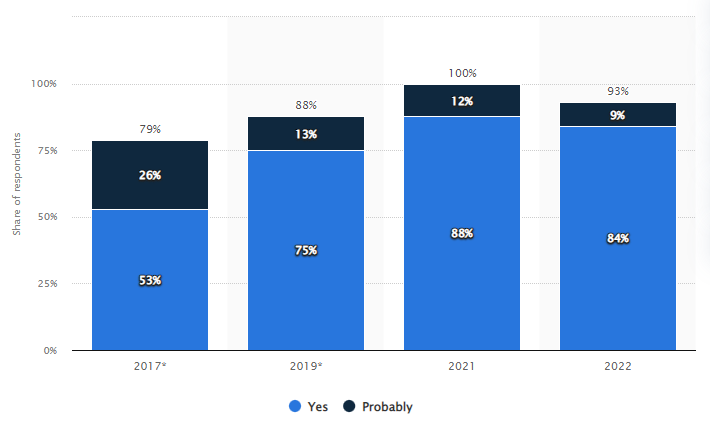
\includegraphics[width=1\textwidth]{gfx/Picture/Cyber_Crime.PNG}
 \caption{Eine Umfrage von deutschen Unternehmen, die von Daten Diebstahl, Espionage oder Sabotage betroffen waren. \cite{Stat22}}
 \label{fig:Crime}
\end{figure}

Wie man in der Grafik (\ref{fig:Crime}) erkennen kann, waren 88\% der befragten Unternehmen in Deutschland von Datendiebstahl, Espionage oder Sabotage in 2021 betroffen.
In 2022 lag die Zahl bei 84\%.
Wobei man berücksichtigen muss, dass diese Befragung zwischen Januar und März stattgefunden hat und dies daher nur das erste Quartal von 2022 abdeckt.
Aufgrund dessen, dass solche Angriffe wahrscheinlich sind, darf es keine "`Super Accounts"' geben, da diese ansonsten in solchen Angriffen als Schwachstelle ausgenutzt werden können.
Genauso müssen die Strukturen übersichtlich sein, damit es bei einer Überprüfung keine Problem darstellt, festzustellen, welcher Nutzer welche Berechtigungen hat.
Wenn dies nicht der Fall ist, kann es passieren, dass die jeweiligen Nutzer zu viele Berechtigungen haben und dies wäre wieder ein Problem bei Espionage oder Sabotage.
Um dies zu erreichen, gibt es verschiedene Methoden und Konzepte, die die Berechtigungsstrukturen sicher und übersichtlich gestalten.

%
% Section: Ziele
%
\section{Ziel der Arbeit}
\label{sec:intro:goal}
Diese Arbeit ist eine Vergleichsarbeit, bei der verschiedene Konzepte verglichen werden.
Dabei wird auf die folgende Fragestellung in dieser Arbeit eingegangen, \textit{inwieweit man bestehende Berechtigungsstrukturen im Hostbereich verändern und optimieren kann}.
Dazu gibt es drei Unterfragen, welche verwendet werden, um die Problemstellung systematisch zu beantworten.

\begin{itemize}
  \item \textit{Welche Konzepte werden derzeit für Berechtigungsstrukturen verwendet, um diese sicher und übersichtlich zu gestalten?}
  \item \textit{Wie unterscheiden sich die verschiedenen Konzepte?}
  \item \textit{Womit kann man die verschiedenen Konzepte vergleichen?}
\end{itemize}

Die erste Unterfrage wird durch eine Recherche mit verschiedenen Arbeiten im Bereich der Berechtigungsstruktur beantwortet.
Dies soll einen Überblick zum Stand der Technik geben.
Anschließend wurden mehrere Befragungen durchgeführt, um die bestehenden Konzepte nach den Wünschen der Befragten anzupassen.
Darauf basierend werden die bestehenden Methoden geranked und verglichen.
Dies beantwortet die zweite Unterfrage mittels des erstellten Vergleiches.
\newline
Um die dritte Frage zu beantworten, wird ein Schema verwendet, welches als eine Hilfestellung zur Konzeptauswahl dienen wird.
Zum Schluss wird eine Alternative zum bestehenden System vorgestellt.
Dies ist die Arbeit in visueller Form.
\newpage
\begin{figure}[h!]
\hspace*{-3cm}
 \centering
 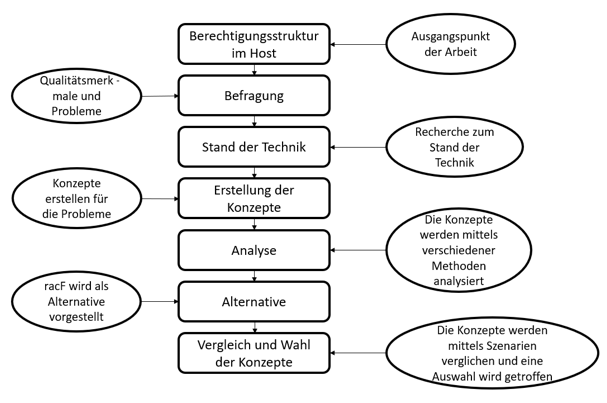
\includegraphics[width=1.5\textwidth]{gfx/Picture/Vorgehen.PNG}
 \caption{Aufbau der Arbeit}
 \label{fig:vorgehen}
\end{figure}
\newpage
\section{Ursache-Wirkungs-Diagramm}
\label{sec:intro:UWD}
\begin{figure}[h!]
 \centering
 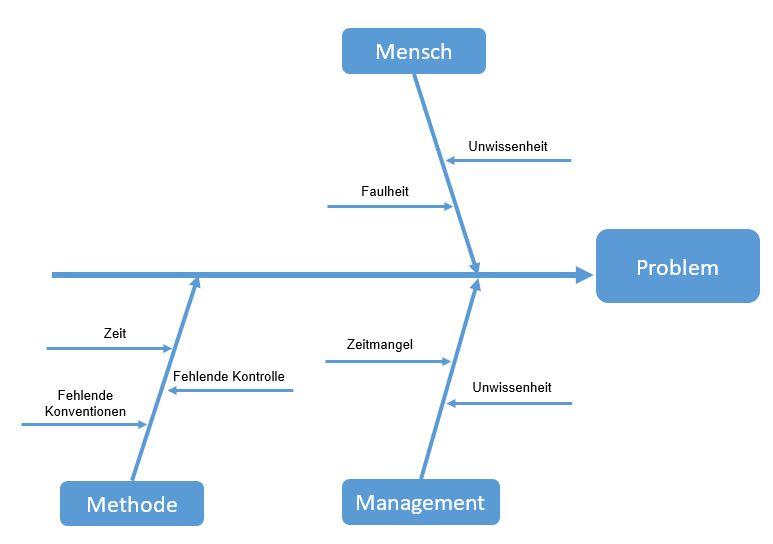
\includegraphics[width=1\textwidth]{gfx/Picture/Fisch.PNG}
 \caption{Ursache-Wirkungs-Diagramm (Fischgrätenmodell)}
 \label{fig:Fisch}
\end{figure}
Im Ursache-Wirkungs-Diagramm wurden dabei die folgenden drei Punkte als Hauptursache für das Problem der bestehenden Berechtigungsstruktur erkannt.
\begin{itemize}
	\item Mensch
	\item Management
	\item Methode
\end{itemize}
Bei Mensch sind die Mitarbeiter genannt, die die Berechtigungsstruktur verwalten und hegen.
Dort wurden die Punkte Faulheit und Unwissenheit genannt.
Dies liegt daran, dass es nicht unüblich ist, dass diese gewisse Formalien ignorieren, um einfacher das Problem zu beheben.
Auf der anderen Seite ist auch die Unwissenheit ein Problem, da die gesamte Struktur so gewachsen ist.
Dadurch ist es unmöglich, für jemand diese komplett nachzuvollziehen.
\newline
Das Management hat nicht die Zeit, sich genau mit dem Problem zu beschäftigen.
Dies hat zur Folge, dass das Management wie die Mitarbeiter unwissend ist.
\newline
Bei der Methode stellt die Zeit, fehlende Kontrolle und fehlende Konventionen als Problem dar.
Mit der Zeit ist gemeint, dass die aktuelle Problemstellung schon so lange der Fall ist, dass dies ein Problem ist.
An vielen Stellen fehlt die Kontrolle bei der bestehenden Berechtigungsstruktur.
Dies ist zum Beispiel der Fall, wenn ein Account wieder aktiviert wird, da dieses nicht überprüft wird.
Denn wenn es diese gäbe, dürfte es keine rekursiven Beziehungen geben.
Es fehlt auch eine allgemeine Konvention, wie die Profile in den verschiedenen Fachbereichen funktionieren.
Dies sorgt dafür, dass es die Mitarbeiter schwerer haben alle Verbindungen zu verstehen und macht die gesamte Struktur komplexer.
\chapter{Definitionen}
\label{ch:chapter02}
Dieses Kapitel erklärt und beschreibt einige der zentralen Begriffe zum Thema des Hosts und der Berechtigungsstrukturen.
Dadurch soll der Leser ein Grundverständnis erhalten, um die folgenden Kapitel zu verstehen.

%
% Section: Der erste Abschnitt
%

\section{Host/Mainframe}
\label{sec:Host}
Der Host bzw. Mainframe ist ein Komplex aus verschiedenen Hochleistungscomputern.
Der Anbieter "`IBM"' definiert diesen dabei wie folgt: 
\newline
\newline
\textit{"`At their core, mainframes are high-performance computers with large amounts of memory and processors that process billions of simple calculations and transactions in real time."'} \cite{Mainframe}
\newline
\newline
Oder übersetzt:
\newline
\newline
\textit{"`Im Kern besteht der Mainframe aus Hochleistungsrechnern, welche über einen großen Speicher verfügen, und in der Lage sind, Milliarden von einfachen Prozessen und Transaktion in Echtzeit durchzuführen."'} \cite{Mainframe}
\newline
\newline
Dabei spielt der Mainframe eine wichtige Rolle in der Finanzindustrie, welche widerstandsfähige, sichere und agile Server benötigt.
Dies ist der Fall, weil die Finanzindustrie über viele sensible Daten verfügt.
Daher müssen die Server sicher und widerstandsfähig sein, damit diese Daten nicht verloren gehen oder gestohlen werden.
Zudem müssen die Server agil sein, da sich die Technologie und die Regulierungen für den Mainframe sich stetig ändern und dieser daher immer auf dem neuesten Stand sein muss.
Der Mainframe muss die Regularien der \ac{VAIT} erfüllen, die von der \ac{BaFin} aufgestellt werden.
Die \ac{BaFin} soll eine konsistente IT-Strategie vorgeben, an die sich die Unternehmen halten müssen. \cite{Vait}

\section{Berechtigung}
\label{sec:Berechtigung}
Dabei definiert die \ac{NIST}, welche eine Institution von der amerikanischer Regierung ist, Berechtigungen wie folgt:
\newline
\newline
\textit{"`The right or a permission that is granted to a system entity to access a system resource."'} \cite{Auth}
\newline
\newline
Dies bedeutet:
\newline
\newline
\textit{"`Das Recht oder die Erlaubnis haben, um auf System Ressourcen einer Systemeinheit zu zugreifen."'} \cite{Mainframe}
\newline
\newline
Im Kontext des Mainframebereiches betrifft dies bei Helvetia hauptsächlich das Betrachten und Zugreifen über Dialogmasken auf Daten.
\begin{figure}[h!]
 \centering
 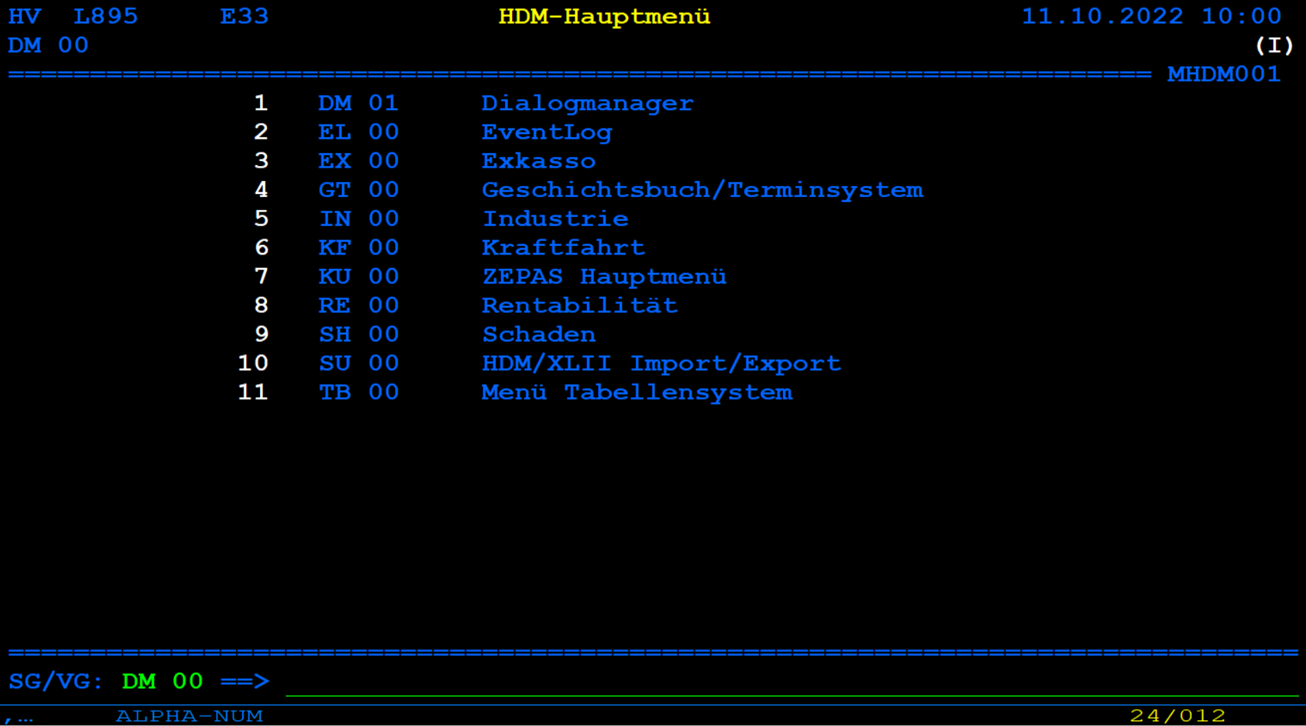
\includegraphics[width=1\textwidth]{gfx/Picture/Dialog.PNG}
 \caption{Beispiel Dialogmaske}
 \label{fig:Dial}
\end{figure}
Die Grafik (\ref{fig:Dial}) zeigt eine solche Dialogmaske.
Anhand dieser Dialogmaske kann man erkennen, dass der Nutzer USER$895$ für die aufgezählten weiteren Dialogmasken (EL$00$, EX$00$, ...) zumindest die Leseberechtigung hat, da diese auf der Dialogmaske DM$00$ angezeigt werden.
Zudem hat dieser die Schreibberechtigungen auf die Dialogmaske DM$00$, da dieser sich in dieser Maske aufhält. 
\newline
\newline
\begin{figure}[h!]
 \centering
 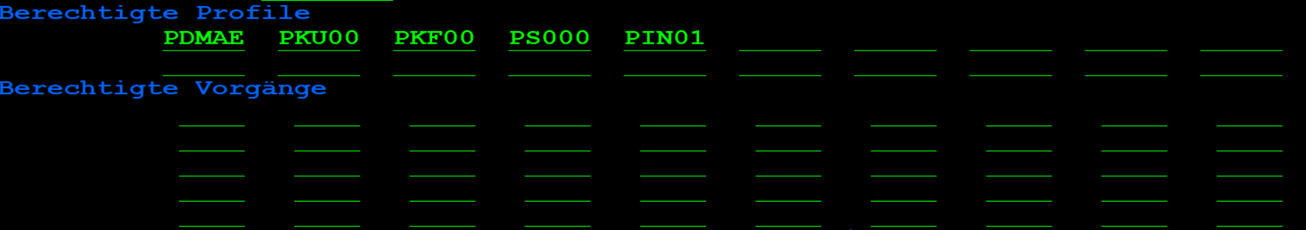
\includegraphics[width=1\textwidth]{gfx/Picture/Berechtigung.PNG}
 \caption{Berechtigungsdialogmaske}
 \label{fig:Berch}
\end{figure}
In dieser Grafik (\ref{fig:Berch}) kann man die Profile und individuellen Berechtigungen sehen, die der Nutzer USER$895$ besitzt.
Dabei sind Profile eine Ansammlung von Berechtigungen.

\section{Berechtigungsstruktur}
\label{sec:Berechtigungsstruktur}
Eine Berechtigungsstruktur besteht aus den Berechtigungen, die im Unterkapitel (\ref{sec:Berechtigung}) definiert werden, und aus der Struktur.
Dabei definiert Oxford Struktur wie folgt:
\newline
\newline
\textit{"`the way in which the parts of something are connected together, arranged or organized; a particular arrangement of parts"'} \cite{Struct}
\newline
\newline
Dies bedeutet, dass die Teile miteinander verknüpft, angeordnet oder organisiert sind. \cite{Struct}
\newline
In diesem Zusammenhang bedeutet Berechtigungsstruktur die Verknüpfung, Anordnung oder Organisation von Berechtigungen.
\begin{figure}[h!]
 \centering
 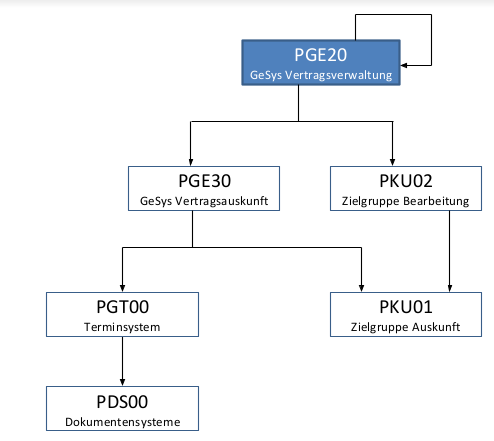
\includegraphics[width=1\textwidth]{gfx/Picture/Struktur.PNG}
 \caption{Teilausschnitt der Berechtigungsstruktur der Helvetia}
 \label{fig:Teil}
\end{figure}
Wie man in der Grafik (\ref{fig:Teil}) erkennen kann, sind die Profile hierarchisch aufgebaut.
Diese Profile beinhalten die Berechtigungen.
\begin{figure}[h!]
\hspace*{-4cm}
 \centering
 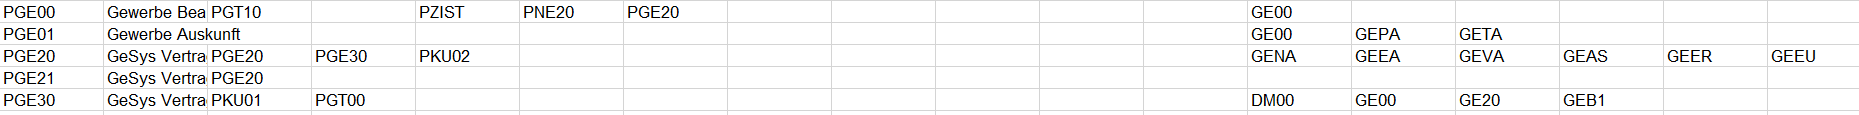
\includegraphics[width=1.6\textwidth]{gfx/Picture/Ber.PNG}
 \caption{Berechtigungen für die Profile PGE$20$ und PGE$30$}
 \label{fig:Ber}
\end{figure}
\newpage
Die Grafik (\ref{fig:Ber}) zeigt, dass die Profile PGE$20$ und PGE$30$ zum Beispiel über die folgenden Berechtigungen verfügen:
\begin{itemize}
	\item DM$00$
	\item GEEA
	\item GEVA
	\item GE$20$
\end{itemize}
Daher ist die aktuelle Berechtigungsstruktur hierarchisch bei der Helvetia.


\section{IAM}
\label{subsec:IAM}
Die Virginia IT Agency beschreibt IAM wie folgt: Das \ac{IAM} ist eine Möglichkeit, sämtliche Nutzer und Profile, welche man zu den jeweiligen Personen über die IT-Umgebung über Nutzerrollen und Businessregeln zu ordnen kann, zu handhaben. Dabei ist die Zugriffverwaltung die Möglichkeit die Zugriffskontrolle über Regeln auf verschiedenen Plattformen einzuhalten. Ein wichtiger Teil von \ac{IAM} ist sicherzustellen, dass die Nutzer einen sicheren Zugriff auf die Ressourcen haben und auch nur auf die Ressourcen, die sie benötigen, um ihre Arbeit zu erledigen. \cite{Virg07} (S. 3)
\begin{figure}[h!]
 \centering
 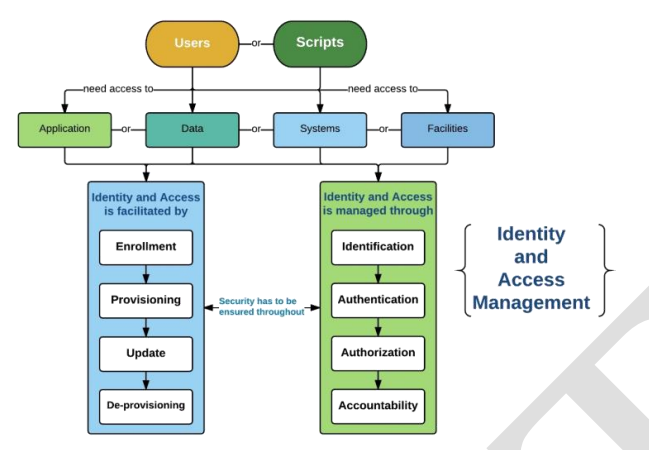
\includegraphics[width=1\textwidth]{gfx/Picture/IAM.PNG}
 \caption{Übersicht von IAM \cite{Moha19}}
 \label{fig:IAM}
\end{figure}
Im Bild (\ref{fig:IAM}) kann man erkennen, dass wenn ein Nutzer oder Programm Zugriff auf eine Ressource möchte, dieser die Identifizierung, Authentifizierung, Autorisierung, sowie Rechtschaffenheit vorlegen und einhalten muss. \cite{Moha19}
Wenn der Nutzer Lucas Stumm beispielsweise die Daten vom Host haben möchte, muss dieser durch verschiedene Schritte gehen.
Als Erstes muss sich dieser Identifizieren mittels eines Nutzernamens und Passworts.
Während dieser sich durch die Menüs manövriert , wird überprüft, ob Lucas Stumm überhaupt die Berechtigungen hat, diese Menüs sehen und auswählen zu können.
Wenn dies der Fall ist, kann der Nutzer auf die Daten zugreifen.
\newline
Im Rahmen dieser Ausarbeitung handelt es sich bei den Ressourcen um die Berechtigungen (\ref{sec:Berechtigung}).

\chapter{Recherche}
\label{ch:Recherche}
In diesem Kapitel geht es um mehrere selbstdurchgeführte Befragungen zur Berechtigungsstruktur und der jährlichen Rezertifizierung.
Die jährliche Rezertifizierung ist die Überprüfung, ob die Mitarbeiter ihre Berechtigungen benötigen oder nicht.
Diese wird von den Teamleitern und Führungskräften durch geführt, welche die Berechtigungstruktur nutzen, um dies zu tun.
Dafür wurden drei verschiedene Gruppen befragt.
Die Ergebnisse sind die Grundlage für die Notwendigkeit eines sicheren und übersichlichen Struktur sowie die Festellung der Hauptprobleme der bestehenden Struktur.

\section{Vorgehensweise}
\label{sec:Vorgehensweise}
Für die Befragung wurde erstmal analysiert welche Stakeholder es gibt.
Bei der Analyse wurden die folgenden drei Stakeholder festgestellt:

\begin{itemize}
	\item \ac{FuT}
	\item Entwickler
	\item Mitarbeiter
\end{itemize}
Die \ac{FuT} entsprechen den Stakeholdern, die die Berechtigungsstruktur für die jährliche Rezertifizierung nutzen.
Diese haben für eine hohe Priorität, da diese die Berechtigungsstruktur direkt verwenden und für die Sicherheit der Struktur gewähren.
\newline
Die Entwickler sind die Stakeholder, die an der Berechtigungsstruktur gearbeitet haben.
Ebenso wie die Teamleiter und Führungskräfte haben die Entwickler auch eine hohe Priorität, weil diese die Struktur warten und verändern.
\newline
Die Mitarbeiter umfassen das restlichen Arbeitspersonal.
Im Gegensatz zu den anderen beiden Stakeholder haben die Mitarbeiter eine geringe Priorität, da diese weder die Struktur nutzen noch einen anderen Kontakt haben.
\newline
\newline
Nachdem diese drei Stakeholder festgestellt worden sind, wurde spezifisch für diese drei Fragenkataloge entwickelt.
Dabei ist das Ziel festzustellen, welche die größten Probleme aus der Sicht der Teamleiter und Führungskräfte sowie Entwickler gibt.
Die Mitarbeiter wurden befragt, wie viele Berechtigungen diese verfügen, die sie eigentlich nicht mehr brauchen.
Die große Herausforderung besteht dabei, die richtigen Fragen für die Fragenkataloge zu entwerfen.
Die Institution \ac{PRC} hat festgestellt, dass bei geschlossenen Fragen die befragt zu einem großen Teil (über 90\%) eine der vorgeschlagenen Antwortet gewählt haben. \cite{Survey}
Dies stellt ein Problem dar.
Wenn die Fragen zu geschlossen sind, dann kann es dazu führen, dass die befragten nicht die Probleme angeben, die sie sehen.
Auf der anderen Seite sind zu offene Fragen auch eine Herausforderung, da es schwierig wird die verschiedenen Antworten zu quantifizieren und auswerten zu können.
Ebenso ist die Wortwahl ein entscheidener Faktor.
In einer Studie von \ac{PRC} in 2003 wurden die Personen befragt, ob diese für oder den Krieg in Iraq sind, um Saddam Hussein's herrschaft zu beenden.
68\% haben ja gesagt und 25\% für nein.
Darauf wurde die Frage geändert zu, ob diese für oder den Krieg in Iraq sind, um Saddam Hussein's herrschaft zu beenden, selbst wenn es tausende Verluste gibt.
Mit dieser Änderung haben nur noch 43\% dafür gestimmt und 48\% dagegen. \cite{Survey}
\newline
Dies ist relevant, da zum Beispiel bei der Befragung der Mitarbeiter bei einer falschen Formulierung den Gedanken bekommen könnten, dass diese mit der Beantwortung der Frage ihr in Ordnung geben, dass ich ihnen die genannten Berechtigungen entfernen.
Dies kann zu fehlerhaften Ergebnissen führen.
Deshalb müssen die Fragen gut überlegt sein.
\newline
\newline
Für die \ac{FuT} wurden die folgenden Fragen überlegt: 
\begin{itemize}
	\item Wie handhabbar ist für Sie der aktuelle Prozess für die jährliche Rezertifizierung der Vorgangsberechtigung Ihrer Mitarbeiter?
	\item Was finden Sie im aktuellen Rezertifizierungsprozess gut?
	\item Was finden Sie im aktuellen Rezertifizierungsprozess schlecht?
	\item Was würden Sie gerne am aktuellen Rezertifizierungsprozess ändern?
	\item Was halten Sie von der Idee das Profile entweder nur noch (Unter-)Profile oder Profile ausschliesslich Berechtigungen beinhalten?
	\item Soll es eine einheitliche Strukturierung für die Berechtigungsstruktur innheralb der Bereiche geben?
	\item Haben Sie weitere Anmerkungen?
\end{itemize}
Die Fragen wurden größtenteils offen Formuliert, um am besten die Probleme am bestehenden System zu finden.
Dabei umfassen die ersten drei Fragen den Ist-Zustand der Berechtigungstruktur und wie dies die \ac{FuT} finden.
Fragen vier, fünf und sechs wie der Soll-Zustand der Berechtigungstruktur werden soll.
Dabei wurden auch konkrete Vorschläge in den Fragen unterbreitet, um einen erst Eindruck von den \ac{FuT} zu erhalten.
Zum Schluss gab es noch die offene Frage, ob es weitere Anmerkungen gibt, um eventuelle Antworten und Anmerkung zu erhalten, die durch die vorherigen Fragen nicht abgedeckt wurden.
\newline
\newline
Für die Entwickler wurden die folgenden Fragen überlegt: 
\begin{itemize}
	\item Welche Erfahrung haben Sie mit der Berechtigungsstruktur gehabt?
	\item Auf welche Probleme sind Sie im Zusammenhang mit der Berechtigungsstruktur gestoßen?
	\item Gibt es Sachen, die man bei der Berechtigungsstruktur beachten muss?
	\item Haben Sie Vorschläge wie man die Berechtigungsstruktur besser gestalten könnte?
	\item Haben Sie weitere Anmerkungen?
\end{itemize}
Die erste Frage soll dazu Anregen sich über das Thema Gedanken zu bilden, damit die folgenden Fragen einfacher zu beantworten sind.
Dabei soll die zweite Frage klarstellen welche Herausforderungen die befragte Person mit der Struktur hatte.
Dies ermöglicht es dann präventiv gegen diese Vorzugehen und dies direkt mit in die neuen Konzepte zu integrieren.
Bei der dritten Frage sollen mögliche ausnahme Fälle genannt werden, die bei einem Konzept mit berücksichtigt werden müssten.
Anschließend wird gefragt, ob die Person eventuel sich selber Gedanken gemacht hat, welche Möglichkeiten es gibt, um die aktuelle Struktur zu verbessern.
Zum Abschluss wird wieder gefragt, ob es weitere Anmerkung gibt, um falls es solche gibt aber nicht von den vorherigen Fragen abgedeckt wurde.
\newline
\newline
Die Mitarbeiter haben die Frage bekommen:
\newline
\newline
\textit{Wie viele Vorgangsberechtigungen in der Produktion Sie im Hoblink haben, die Sie nicht mehr nutzen?}
\newline
\newline
Bei dieser Frage ware es wichtig diese so zu formulieren, dass die befragte Person nicht den Eindruck bekommt, dass ich ihr die Berechtigungen wegnehmen möchte.
Dies würde ansonsten zu fehlerhaften Ergebnissen führen.
Die Befragung der Mitarbeiter dient dazu, um die Problematik der nicht optimalen Berechtigungsstruktur darzustellen und auch um feste Zahlen zu haben.

\section{Auswertung}
\label{sec:Auswertung}


\section{Ergebnis}
\label{sec:Ergebnis}
\chapter{Konzepte}
\label{ch:chapter04}
In diesem Kapitel wird darauf eingegangen, wie vorgegangen wurde, um verschiedene Konzepte zu entwickeln.
Dabei werden die vorher erwähnten Befragungen (\ref{ch:Recherche}) verwendet, um eine Lösung für die individuellen Probleme zu entwickeln.
Zudem wird der Stand der Technik betrachtet und ein Vergleich mit den Datenbankstrukturen gezogen.
Dies wird getan, da diese eine ähnliche Struktur wie die Berechtigungsstruktur der Helvetia haben. 
Anschließend werden die Probleme aus den Befragungen quantifiziert, um daraus die verschiedenen Konzepte zu entwickeln.

\section{Konzeptentwicklung}
\label{sec:chapter04:Konzeptentwicklung}
In diesen Unterkapiteln wird betrachtet, was der Stand der Technik ist.
Dabei werden die Sicherheitsmaßnahmen von \ac{IAM} erläutert sowie berücksichtigt, dass es nicht die eine Lösung für das Problem gibt.
Zudem wird auch erläutert, wie die Berechtigungsstruktur innerhalb von Datenbanken funktioniert, um diese als einen Vergleich zu nutzen.  

\subsection{Stand der Technik}
\label{sec:chapter04:Stand}
In der Welt von Cloud Computing wird \ac{IAM} als Sicherheitsmaßnahme verwendet.
Dabei wird mittels \ac{IAM} die Identität und der Zugriff reguliert.
\ac{IAM} kann daher in die folgenden fünf Punkte gegliedert werden.
\newline
\newline
1. Authentifizierung der Person
\newline
Dabei wird überprüft, ob die Person auch wirklich, die ist, als welche diese sich ausgibt.
Um dies sicherzustellen, gibt es verschiedene Methoden.
Ein Nutzername mit einem Passwort ist hierbei die gängigste Methode, um dies zu tun. Dies wird von den meisten Webseiten und Computern verwendet.
Um die Authentifizierung sicherer zu gestalten, werden mehrere Faktoren berücksichtigt, die eine Person identifizieren.
Dies kann zum Beispiel durch einen Fingerabdruck stattfinden. \cite[1482]{IamIEEE} 
\newline
\newline
2. Berechtigungsvergabe
\newline
Die Berechtigungsvergabe beschäftigt sich damit, welche Berechtigungen jeder Nutzer bekommt.
Dies wird mittels Autorisierungsrichtlinien gesichert, damit die Nutzer nur Zugriff auf die Ressourcen und Dienste haben, welche sie benötigen.
Dies wird mithilfe von Profilen erreicht, welche ihnen von der Organisation zugewiesen werden. \cite[1482]{IamIEEE} 
\newline
\newline
3. Identitätsvergabe
\newline
Die Identitätsvergabe sorgt dafür, dass der Nutzer eine digitale ID oder einen Account erhält.
Wenn ein Mitarbeiter bei einem Unternehmen arbeitet, erhält dieser eine digitale Identität, um auf die Ressourcen des Unternehmens zugreifen zu können.
Dabei ist auch wichtig, dass der Mitarbeiter diese digitale Identität wieder verliert, wenn dieser das Unternehmen verlässt oder an einer anderen Stelle im Unternehmen arbeitet und seine alte digitale Identität nicht mehr benötigt. \cite[1482]{IamIEEE}
\newline
\newline
4. Föderierte Identität
\newline
Dabei handelt es sich darum, dass die digitalen Identitäten über verschiedene Anwendungen und Organisationen gültig sind.
Dafür werden die Informationen der digitalen Identität gespeichert.
Dies hat den Vorteil, dass der Nutzer sich nur einmal anmelden muss, um auf sämtliche seiner Ressourcen zugreifen zu können.
Dabei werden Protokolle wie SAML, OAuth oder OpenID verwendet.
Die Folge dadurch ist, dass der Nutzer sich nicht mehrere Passwörter sowie Accounts merken muss. \cite[1482]{IamIEEE}
\newline
\newline
5. Compliance Verwaltung
\newline
Die Compliance Verwaltung überprüft die Authentifizierungs- und Zugriffsaufzeichnungen, um sicher zu stellen, dass die Richtlinien und Sicherheitsstandards eingehalten wurden.
Diese Überprüfung ist notwendig für effektive Zugriffsregeln.
Zudem werden diese für Audits benötigt. \cite[1482]{IamIEEE} 
\newline
\newline
\begin{figure}[h!]
 \centering
 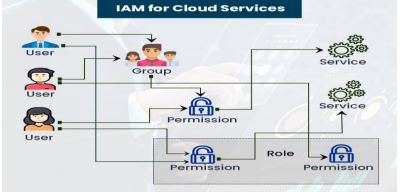
\includegraphics[width=1\textwidth]{gfx/Picture/IAMISH.PNG}
 \caption{IAM für Cloud Dienste \cite[3]{Moha19}}
 \label{fig:IMAISH}
\end{figure}
Dies ist ein Beispiel, wie die oben genannten Punkte umgesetzt werden können.
Dabei haben die Accounts der Personen entweder direkte Berechtigung oder diese werden mittels Gruppen verteilt.
Sobald der Account die Berechtigung hat, kann dieser auf die dahinter steckende Ressource zugreifen.
Die Berechtigungen können dabei auch mittels Profile zusammengefasst werden.
Die Grafik (\ref{fig:IMAISH}) stellt dies dar.
\newline
Dabei kann dies auf verschiedenen Wegen umgesetzt werden, da dieselbe Lösung für gewisse Fälle nicht funktioniert.
Zum Beispiel beschreibt \cite[208]{Cal17} das Problem, wie die United States of America am besten mit ihren Verbündeten kooperieren sollten.
Da es sich dabei um sensitive Informationen handelt, welche an verschiedene Partner vermittelt werden, muss der Zugriff reguliert werden.
Auch haben die verschiedenen Länder unterschiedliche Gesetze, worauf geachtet werden muss. 
Deswegen gibt es keine universelle Methode, um eine solche Herausforderung zu lösen. \cite[208]{Cal17}


\subsection{Vergleich mit Datenbanken}
\label{sec:chapter04:DB}
Die Helvetia verwendet zum Speichern der Informationen für die Berechtigungsstruktur sogenannte HV-Tabellen.
Bei diesen HV-Tabellen handelt es sich, um DB$2$-Tabellen.
Zudem besteht eine Ähnlichkeit zwischen dem Nutzer und dem Profil in der Berechtigungsstruktur im Vergleich zum Account und der Gruppe in Datenbanken.
Deswegen wird betrachtet, wie der Standard von Accounts und Gruppen innerhalb von Datenbanken ist.
\newline
Berechtigungen für Rollen werden mittels folgenden Kommand vergeben: 
\newline
\newline
GRANT...ON...TO...[GRANT OPTION]
\newline
\newline
Dabei wird für die spezifische Berechtigung, zum Beispiel eine View und einen Account oder eine Gruppen angegeben.
Zudem kann auch hinzugefügt werden, ob die Rolle die Berechtigung hat, anderen Accounts die Berechtigungen zu geben.\cite[474-475]{Ram09}
\newline
Wenn man sich zum Beispiel das Bild (\ref{fig:Berch}) ansieht, könnte der Befehl wie folgt aussehen:
\newline
\newline
GRANT UPDATE ON PKU$00$ TO USER$895$.
\newline
\newline
Das würde in diesem Beispiel bedeuten, dass der Nutzer USER$895$ die Bearbeitungsberechtigung für die Ressource PKU00 erhalten hat.
Dabei ergibt sich die Frage auf, was bevorzugt verwandt werden sollte:
\newline
Eine individuelle Berechtigungsvergabe oder Gruppenvergabe für die Accounts.
Microsoft hat folgendes als Best Practice definiert:
\newline
\newline
\textit{"`To simplify administration, create groups and assign each group permission to functional areas and model objects.
You can then add and remove users from the groups without accessing the Master Data Manager UI.
\newline
\newline
Do not assign additional permissions to an individual user, and do not include a user in multiple groups that have access to Master Data Manager. In addition, do not use hierarchy member permissions unless you want a group to have limited access to specific members."'} \cite{Micro}
\newline
\newline
Microsoft gibt an, dass man Gruppen erstellen soll.
Die individuellen Nutzer sollen dabei keine zusätzlichen Berechtigungen bekommen.
Ebenso ist es wichtig, dass diese nicht in mehreren Gruppen sind, welche Zugriff auf den Master Data Manager haben.
Und auch IBM gibt in seiner Best Practice an, dass Angestellte in einem Unternehmen mittels Gruppen organisiert werden sollten. \cite{IBMGroup}
\newline
Dies ist jedoch in der Praxis schwierig umzusetzen.
Im Idealfall benötigt jeder Mitarbeiter ein oder zwei Standardprofile, welche dem Nutzer alle Berechtigungen geben.
Dies ist aber selten der Fall, da die Nutzer nach beispielsweise einem halben Jahr an einem anderen Projekt arbeiten und daher andere Berechtigungen benötigen.
Wenn man für jeden solchen Fall ein neues Standardprofil erstellt, werden diese unübersichtlich.
Ebenso würde das Konzept der Standardprofile in Frage gestellt werden, wenn die Anzahl dieser Standardprofile der Anzahl der Berechtigungen gleicht.
Dennoch sollte es versucht werden, dass Nutzer so wenig zusätzliche Berechtigungen wie möglich bekommen, um Best Practice Standards einzuhalten. 

\section{DSGVO}
\label{sec:chapter04:DSGVO}
Neben den technischen Herausforderungen und Anforderungen muss die Struktur neben dem \ac{VAIT} auch den Standards der \ac{DSGVO} erfüllen.
Bei Verstoß gegen diese kann es zur Verwarnung bis zum endgültigen Verbot der Datenverarbeitung kommen. \cite{EuroK}
Dies würde die Helvetia sehr viel Geld kosten, da diese nicht mehr operieren könnte.
\newline
Eine sichere Berechtigungsstruktur ist daher nötig, um diese Anforderung der \ac{DSGVO} zu befriedigen.
Diese ist nämlich verletzt, wenn Daten, für die das Unternehmen verantwortlich ist, in ihrer Vertraulichkeit, Verfügbarkeit oder Integrität verletzt werden.
Deswegen sind Mitarbeiter, die mehr Berechtigungen haben als jene, die sie wirklich benötigen, eine Risikostelle. \cite{EuroW}
\newline
Daher sollte die neue Berechtigungsstruktur so gestaltet werden, dass die Verständlichkeit, Verfügbarkeit und Integrität der Daten nicht verletzt werden können.

\section{Herausforderung und Anforderungen}
\label{sec:chapter04:Herausforderung}
Bei der Recherche (\ref{ch:Recherche}) sind verschiedene Herausforderungen und Anforderungen aufgetreten.
Um qualitativ ein Konzept entwickeln zu können, müssen diese Herausforderungen und Anforderungen aufgelistet und analysiert werden.
Neben den genannten Punkten wurde der Punkt Implementierung hinzugefügt, da diese bei der Entscheidung der Konzepte elementar ist.
Das Unternehmen muss sich dabei über die Kosten des neuen Konzepts und dessen Performance bewusst sein.
\begin{itemize}
	\item Performance der Tabellen erhöhen 
	\item Übersichtlichkeit erhöhen (effizientere Verifizierung der Mitarbeiter)
	\item Rekursive Beziehungen verhindern
	\item Hierarchien verringern
	\item \ac{K/W}
	\item Implementierung
\end{itemize}
Eine Quantifizierung findet mittels Prioritätsanalyse (\ref{fig:Prio}) statt, um festzustellen, wie die Prioritäten der Konzepte zu bewerten sind. \cite{BdIufH}
Bei der Prioritätsanalyse wurde sich für ein vier Punktesystem entschieden.
\newline
Im Vergleich zwischen der Performance und der Übersichtlichkeit wurden der Performance drei Punkte gegeben und die Übersichtlichkeit hat nur einen Punkt erhalten, da die Performance eine der Grundanforderungen ist, weswegen die Berechtigungsstruktur geändert werden soll.
Die Übersichtlichkeit dazu ist weniger wichtig.
Die Performance und die Rekursion haben jeweils zwei Punkte bekommen, da eine performante Struktur keine rekursiven Beziehungen enthält.
\ac{K/W} sowie Performance haben jeweils zwei Punkte bekommen.
Dies liegt daran, dass neben der Performance die \ac{K/W} elementar sind, da eine Struktur, die sich kaum warten lässt, mehr Ressourcen in der Zukunft kosten wird.
Dabei haben die Performance und Hierarchie jeweils zwei Punkte erhalten.
Zwischen der Übersichtlichkeit und der Rekursion wurden der Rekursion drei Punkte gegeben und der Übersichtlichkeit nur einen, weil rekursive Strukturen unübersichtlicher sind und es daher wichtiger ist, dass es keine gibt.
Übersichtlichkeit und Hierarchie haben beide zwei Punkte erhalten, da beide eine gleiche Rolle bei der Lesbarkeit der Struktur spielen.
Übersichtlichkeit sowie Rekursion und Hierarchie bekommen einen Punkt im Vergleich zu \ac{K/W}, weil dieser Punkt langfristig eine wichtige Rolle spielt, und die anderen drei Punkte sollten keine Probleme sein, sofern sich an die Konventionen gehalten wird, damit die Struktur wartbar bleibt.
Die Rekursion bekommt zur Hierarchie vier Punkte und die Hierarchie zur Rekursion null Punkte, da eine rekursive Beziehung die Hierarchie automatisch unendlich macht.
\newline
\newline
Wenn man dies auswertet, bekommt die Performance einen Gewichtsfaktor von 16,67\%, die Übersichtlichkeit 20,00\%, die Rekursion 18,33\%, die Hierarchie 6,67\%, die \ac{K/W} 18,33\% und Implementierung 20,00\%.
Dadurch sieht die Rangfolge wie folgt aus:
\begin{enumerate}
	\item Implementierung | Übersichtlichkeit
	\item Rekursion | \ac{K/W}
	\item Performance
	\item Hierarchie
\end{enumerate}
Anhand dieser Reihenfolge werden die folgenden Konzepte entwickelt.
\newpage
\begin{figure}[h!]
\hspace*{-2cm}
 \centering
 \includegraphics[width=1.25\textwidth]{gfx/Picture/Prioritatätsanalyse.PNG}
 \caption{Prioritätsanalyse der Kriterien}
 \label{fig:Prio}
\end{figure}

\section{Konzept hierarchische Struktur}
\label{sec:chapter04:Struktur}
\begin{figure}[h!]
 \centering
 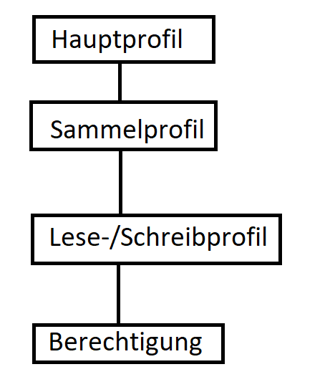
\includegraphics[width=0.75\textwidth]{gfx/Picture/Hierarchie.PNG}
 \caption{Hierarchieaufbau für das Konzept hierarchische Struktur}
 \label{fig:Struktur}
\end{figure}
Das erste Konzept für die Struktur ist wie folgt aufgebaut.
Wie man in der Grafik (\ref{fig:Teil}) aus dem zweiten Kapitel erkennen kann, gibt es bei der aktuellen Berechtigungsstruktur keine Struktur.
Um dementsprechend die genannten Problem zu beheben, wurde die neue Struktur (\ref{fig:Struktur}) entwickelt.
Um die \ac{K/W} zu verbessern, wurden die folgenden Konventionen für dieses Konzept entwickelt.
Es ist dabei anzumerken, dass die Durchsetzung und Implementierung dieser Konventionen trotzdem keinen unerheblichen Aufwand darstellt.
\begin{itemize}
	\item Profile enthalten nur noch Profile oder Berechtigungen.
	\item Die Berechtigungsstruktur soll nur noch eine Hierarchietiefe von maximal vier Ebenen haben.
	\item Die erste Hierarchiestufe enthält das Standardprofil, welches dem Nutzer gegeben wird.
	\item Die zweite Hierarchiestufe enthält die jeweiligen Sammellese- und -schreibprofile, die jeweils in die Fachbereiche getrennt sind.
	\item Die dritte Hierarchiestufe enthält die individuellen Lese- und Schreibprofile.
	\item Die vierte Stufe enthält die Berechtigungen.
	\item Manche der bestehenden Profile beinhalten aktuell, was zukünftig Hauptprofile wären.
In solchen Fällen würden diese Profile zu Hauptprofilen werden und vom vorherigen Hauptprofil separiert werden.
	\item Manche Fachbereiche haben aufzählende Profile (\ref{fig:Profile}).
Diese Profile sollen nur noch die Berechtigungen für den eigenen Vorgang enthalten, sodass ein Privas Profil nur Privas Berechtigungen enthält.
Die Berechtigungen, die verloren gehen, würden eigene Profile bekommen und so über ein anderes Sammelprofil dem Hauptprofil hinzugefügt werden.
	\item Sollte ein Nutzer weitere Berechtigungen benötigen, würden ihm diese direkt zugewiesen werden.
	\item Wenn ein Account reaktiviert wird, muss dieser rezertifiziert werden.
\end{itemize}
Diese Konventionen sollen verhindern, dass die Struktur weiter wächst und dass man ohne Probleme feststellen kann, was für Berechtigungen ein Profil hat.
Zudem hat es den Vorteil, dass rekursive Beziehungen sowie redundante Berechtigungsvergabe nicht möglich sind, da die Profile nur noch Profile oder Berechtigungen enthalten, die nicht mehr auf sich gegenseitig zeigen.
Die Verschachtelung der Profile sorgt nämlich dafür, dass die Gesamtstruktur unübersichtlich wird. \cite[21]{RuB}
Dadurch soll auch die Übersichtlichkeit verbessert und das Hierarchieproblem auf ein Minimum gebracht werden.
Außerdem sollte die Performance verbessert werden.
Dabei helfen verschiedene Faktoren, um diese zu verbessern.
Die Reduktion der rekursiven Beziehungen, sowie die Vereinfachung der Struktur, mit der Reduktion der Berechtigungen, machen die Berechtigungsstruktur performanter.
Diese Standardprofile sollten idealerweise, die einzigen sein, welche die Nutzer benötigen. \cite[21]{RuB}
Leider ist dies in Praxis nicht immer umsetzbar, da die Aufgaben der Nutzer sich ändern können.
Trotzdem versucht das Konzept das Prinzip vom Least Privilege umzusetzen.
Dabei geht es darum, dass der Nutzer nur die Berechtigungen erhält, welche dieser benötigt. \cite[1]{LePr}

\begin{figure}[h!]
\hspace*{-2cm}
 \centering
 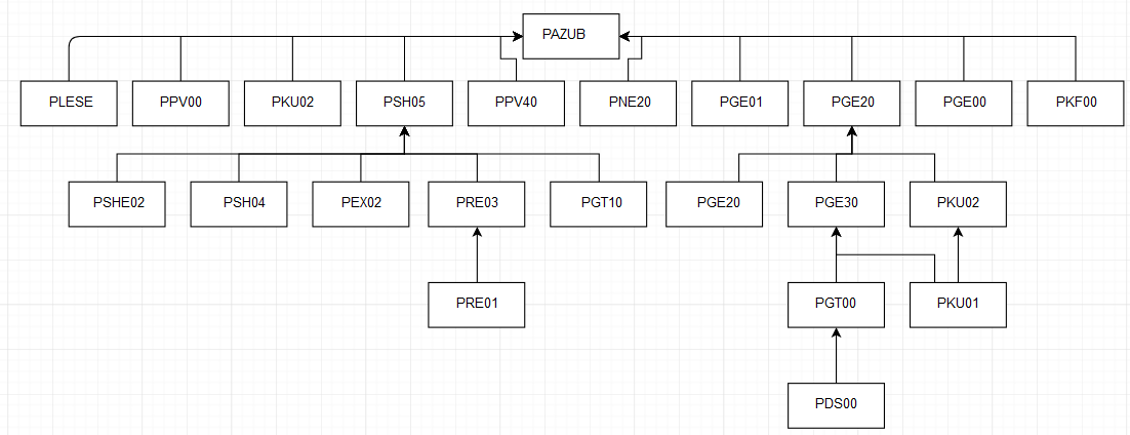
\includegraphics[width=1.25\textwidth]{gfx/Picture/Vorher.PNG}
 \caption{Beispiel der bestehenden Berechtigungsstruktur}
 \label{fig:AltBer}
\hspace*{-2cm}
 \centering
 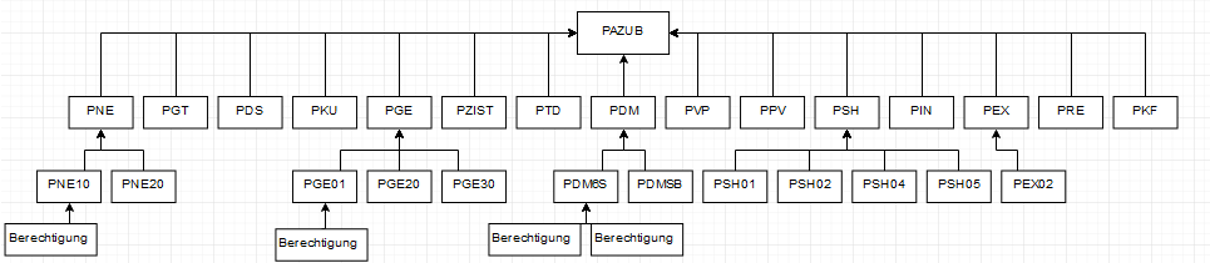
\includegraphics[width=1.25\textwidth]{gfx/Picture/Nachher.PNG}
 \caption{Beispiel der neuen Berechtigungsstruktur}
 \label{fig:NeuBer}
\end{figure}
Das Bild (\ref{fig:AltBer}) zeigt eine bestehende Berechtigungsstruktur.
(\ref{fig:NeuBer}) hingegen bildet die Struktur nach den neuen Konventionen dar.
Diese beiden Bilder wurden den befragten IT-Spezialisten gezeigt.
Einheitlich haben alle befragten IT-Spezialisten angegeben, dass Sie die neue Struktur übersichtlicher finden und diese einfacher zu verstehen ist.
Zudem wurde auch erkannt, dass die Hierarchie verringert wurde.
\newline
Das aktuelle Verfahren, das verwendet wird, um die Berechtigung zu überprüfen, gleicht einem Insertion-Sort.
Dabei wird jedes einzelne Profil durchgegangen, bis die gewünschte Berechtigung gefunden wurde.
Dies weißt eine Komplexität von n im Optimalfall und $n^2$ im schlimmsten Falle auf.
n beschreibt dabei die Anzahl von Profilen/Berechtigungen, die der Algorithmus durchlaufen muss. \cite[12]{log} \cite{weblogMer}
\newline
Bei der neuen Struktur kann ein Merge-Sort genutzt werden.
Dabei achtet der Algorithmus auf bestimmte Eigenschaften der Profile.
Würde zum Beispiel verlangt werden, dass der Nutzer eine Berechtigung für PNE10 hat, würde nur der Baum von PNE durchsucht werden und in diesem Falle direkt PNE10 ausgewählt werden.
Dieser Suchalgorithmus ist komplexer als der Insertion-Sort. Er ist jedoch deutlich effizienter bei einer größeren Menge von Profilen und Berechtigungen.
Die Komplexität beläuft sich bei ihm auf n*log(n) im besten, wie auch im schlechtesten Fall. \cite[12]{log} \cite{weblogMer}
\newline
Wenn beispielsweise n = $100$ wäre, würden die Ergebnisse wie folgt aussehen:
\newline
\newline
Best-Case(Insert) = $100$
\newline
Worst-Case(Insert) = $100^2 = 10.000$
\newline
\newline
Best-Case(Merge) = $100*log(100) = 200$
\newline
Worst-Case(Merge) = $100*log(100) = 200$
\newline
\newline
Wie man erkennen kann, ist der neue Algorithmus im Best-Case langsamer, aber im Worst-Case deutlich schneller und bietet allgemein eine konsistente Zeit, welche für eine Versicherung wichtig ist.
Der Insertion-Sort sowie der Merge-Sort haben auch eine average Formel: \cite{weblogMer,weblogIn}
\newline
\newline
Average(Insert) = $100^2 = 10.000$
\newline
\newline
Average(Merge) = $100*log(100) = 200$
\newline
\newline
Man kann erkennen, dass im normalen Fall die neue Struktur mit dem Merge-Sort deutlich effektiver ist als die bestehende Struktur.
Diese würde durchschnittlich $50$ mal effektiver sein.
\newline
\newline
Die Entwicklung dieses Konzeptes ist aufwendig und komplex.
Es gibt dabei zwei Möglichkeiten, wie dieses umgesetzt werden kann.
Die erste Möglichkeit besteht darin, dass sich eine Gruppe von Entwicklern an die bestehende Struktur setzen, eine Kopie davon erstellen und anhand der Kopie die neue Struktur erstellen.
Dies ist jedoch zeitaufwändig und es besteht ein hohes Potenzial, dass Fehler durch nachlässiges Arbeiten geschehen.
\newline
Die zweite Möglichkeit wäre ein Algorithmus zu schreiben, welcher dies automatisiert.
Da weder die Zeit besteht, noch die entsprechende Umgebung zum Testen eines Prototypen vorhanden ist, kann die Entwicklung des Algorithmus innerhalb dieser Arbeit nur mithilfe von Pseudocode stattfinden.
Dabei würde die Automatisierung wie folgt aussehen.
\newline
\newline
\textbf{Algorithmus} conversionToNewStructure(DB$2$ T)
\newline
\newline
\textbf{Input} Eine DB2 Tabelle T, welche die Struktur enthält
\newline
\newline
\textbf{Output} Neue DB2 Tabelle NT, welche die neue Struktur von Profilen enthält.
\newline
\newline
Der Algorithmus muss dabei die Profile in zwei Kategorien aufteilen:
\begin{itemize}
	\item Standardprofil
	\item Lese-/Schreibprofil
\end{itemize}
Für die Standardprofile werden die Profile überprüft, die viele Unterprofile haben.
Wenn ein Profil XY viele Unterprofile hat, wird dieses zu einem Standardprofil.
Die restlichen Profile werden zu Lese-/Schreibprofile.
Die individuellen Sammelprofile werden basierend auf den Lese-/Schreibprofilen generiert.
Die Verbindungen zwischen den bisherigen Profilen werden aufgebrochen und den neuen Sammelprofilen zugewiesen, welche mit dem Standardprofil verbunden sind.
Anschließend wird auf redundante Profile und Berechtigungen überprüft, welche dann entfernt werden.
Dabei muss man aber zum Schluss begutachten, ob alle generierten Standardprofile wirklich Standardprofile sein sollten sowie ob die bestehende Anzahl ausreichend ist.
Die Grafik (\ref{fig:Hier}) stellt dies als Ablaufdiagram dar.
\begin{figure}[h!]
 \centering
 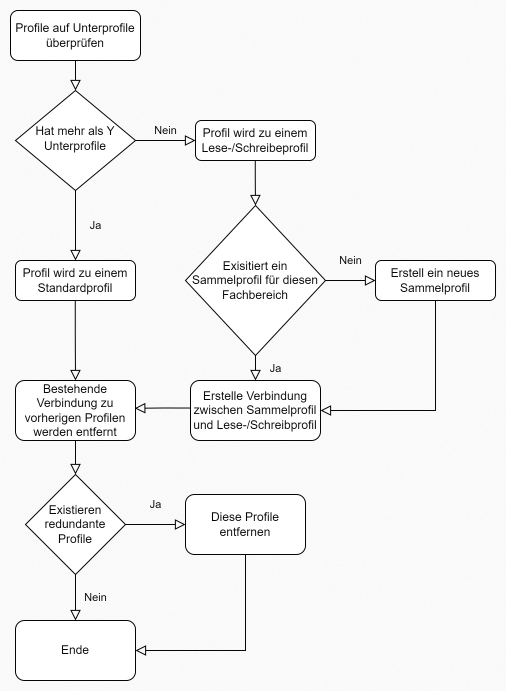
\includegraphics[width=0.77\textwidth]{gfx/Picture/Hier.PNG}
 \caption{Ablaufdiagram für das hierarchische Strukturkonzept}
 \label{fig:Hier}
\end{figure}
\newpage

\section{Konzept minimalistische Struktur}
\label{sec:chapter04:minimal}
Im Gespräch mit den IT-Spezialisten kam der Vorschlag auf, dass man einen minimalistischen Ansatz nutzen könnte.
Dabei haben die IT-Spezialisten folgende Vorschläge für die Konventionen gemacht:
\newline
\begin{itemize}
	\item Profile enthalten nur noch Profile oder Berechtigungen.
	\item Es werden Standardprofile für die jeweiligen Abteilungen entwickelt.
	\item Nutzer, die in verschiedenen Abteilungen operieren, erhalten die jeweiligen Standardprofile.
	\item Zusätzliche Berechtigungen werden dem Nutzer direkt zugeordnet.
	\item Wenn ein Account reaktiviert wird, muss dieser rezertifiziert werden.
\end{itemize}
\begin{figure}[h!]
 \centering
 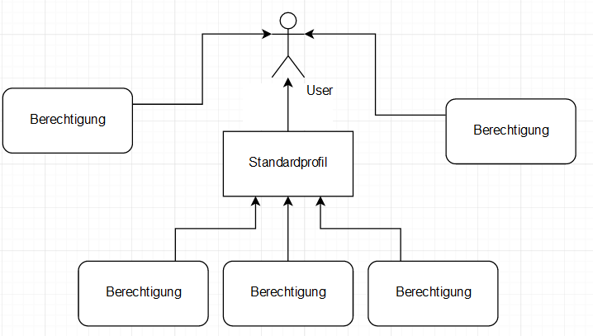
\includegraphics[width=1\textwidth]{gfx/Picture/Minimal.PNG}
 \caption{Darstellung für das Konzept minimalistische Struktur}
 \label{fig:Min}
\end{figure}
Die IT-Spezialisten fanden auch, dass dies übersichtlicher als die bestehende Struktur ist.
Dieses Konzept hat den Vorteil, dass es kaum noch eine Hierarchie gibt.
Dadurch entfällt das Problem der Rekursion sowie redundanter Berechtigungsvergabe.
Ebenso wird das Prinzip des Least Privilege erfüllt, da der Nutzer die zusätzlichen Berechtigungen selbst anfordern muss.
Die \ac{K/W} ist einfacher in diesem Sinne, da nur überprüft werden muss, ob die Standardprofile über die notwendigen Berechtigungen verfügen.
Auf der anderen Seite ist die Entwicklung aufwendig, da erst einmal bestimmt werden muss, welche Berechtigungen für einen Fachbereich notwendig sind.
Ebenso muss sichergestellt werden, dass alle Nutzer ihre Berechtigungen beibehalten.
Es besteht nämlich die Gefahr, dass bei dem Wechsel Berechtigungen verloren gehen.
\newline
\newline
Wenn man (\ref{fig:Min}) betrachtet, kann für diese Struktur nur ein Insertion-Sort verwendet werden.
Dies liegt daran, dass der Sort die individuellen Einträge durchlesen muss, da es keine Information gibt, wo welche Berechtigung ist.
Die aktuelle Struktur verwendet auch einen Insertion-Sort, aufgrund des gleichen Problems.
Jedoch ist zu bemerken, dass die Anzahl der \textit{n} bei diesem Konzept geringer ist, da es nicht die verschiedenen Profile mit Redundanzen gibt.
\newline
\newline
Ein Hauptprofil hatte zum Beispiel $110$ Profile mit enthalten Berechtigungen.
Von diesen $110$ waren $78$ redundante Profile.
Da Profile eine Ansammlung von Berechtigungen sind, ist die Anzahl von redundanten Berechtigungen deutlich höher.
Wenn man nur zwischen der bestehenden Struktur mit der minimalistischen Struktur unterscheidet, erhält man folgenden Vergleich:
\newline
\newline
Best-Case(Alte Struktur) = $110$
\newline
Worst-Case(Insert) = $110^2 = 12.100$
\newline
Average(Insert) = $110^2 = 12.100$
\newline
\newline
Best-Case(Neue Struktur) = $32$
\newline
Worst-Case(Neue Struktur) = $32^2 = 1.024$
\newline
Average(Neue Struktur) = $32^2 = 1.024$
\newline
\newline
Man kann feststellen, dass obwohl die neue Struktur nicht über einen effizienteren Algorithmus verfügt, dieser trotzdem eine bessere Performance hat.
Die neue Struktur wäre in diesem Beispiel ca. $12$ mal performanter als die bestehende Struktur.
\newline
\newline
Ebenso kann für dieses Konzept eine manuelle Lösung sowie auch eine automatische verwendet werden.
Wie im vorherigen Fall kann eine Kopie vom vorherigen Konzept erstellt werden, welche dann in das neue Konzept modeliert wird.
Jedoch wird der Prozess der individuellen Berechtigungsvergabe zu den einzelnen Nutzern zeitaufwendig sein.
Dabei können auch Berechtigungen verloren gehen, was dringend zu vermeiden ist.
\newline
Als Alternative kann ein Algorithmus verwendet werden.
Dieser gleicht, in der Grundstruktur, dem vorherigen Algorithmus:
\newline
\newline
\textbf{Algorithmus} conversionToNewStructure(DB$2$ T)
\newline
\newline
\textbf{Input} Eine DB2 Tabelle T, welche die Struktur enthält
\newline
\newline
\textbf{Output} Neue DB2 Tabelle NT, welche die neue Struktur von Profilen enthält.
\newline
\newline
Der Algorithmus würde die komplette bisherige Struktur auseinanderbrechen.
Anschließend werden die Standardprofile anhand der Fachbereiche neu geformt und den Nutzern der jeweiligen Bereiche zugewiesen.
Die bisherigen Berechtigungen werden anschließend den Nutzern direkt angehängt.
Redundante Berechtigungen werden entfernt.
Die Grafik (\ref{fig:Mini}) stellt dies als Ablaufdiagram dar.
\begin{figure}[h!]
 \centering
 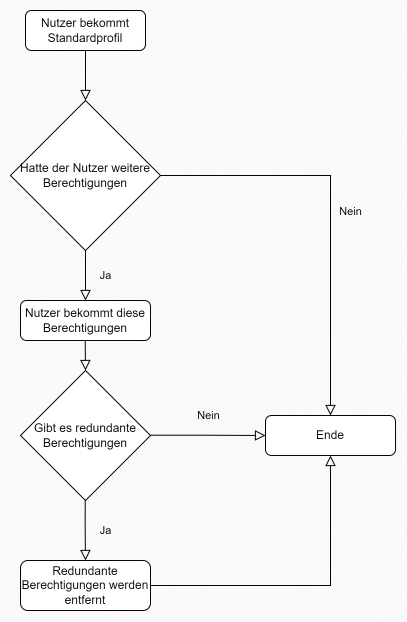
\includegraphics[width=1\textwidth]{gfx/Picture/Mini.PNG}
 \caption{Ablaufdiagram für das minimalistische Konzept}
 \label{fig:Mini}
\end{figure}
\chapter{Fazit}
\label{ch:chapter05}
liquam facilisis convallis nibh. Ut accumsan malesuada nisi, eget luctus ante dignissim at. Integer dignissim rutrum feugiat. Mauris sit amet leo id ligula fringilla pharetra. In id neque metus, eu congue libero. Suspendisse egestas imperdiet nulla, in blandit dolor venenatis vel. Quisque quis justo quis quam lobortis blandit. Quisque urna mauris, placerat a pretium eu, placerat vel risus. Donec sollicitudin malesuada cursus. Sed auctor aliquet urna sit amet porta. Cum sociis natoque penatibus et magnis dis parturient montes, nascetur ridiculus mus. 

\section{Empfehlung}
\label{sec:chapter03:grafiken:minipage}
Donec gravida consequat arcu, et mollis tortor posuere vitae. Sed pharetra turpis a ante commodo accumsan. Suspendisse leo nulla, accumsan sit amet dapibus in, posuere eget turpis. Vivamus enim sapien, porta id placerat eget, laoreet sed massa. Class aptent taciti sociosqu ad litora torquent per conubia nostra, per inceptos himenaeos.

\section{Ausblick}
\label{sec:chapter03:grafiken:minipage}
Donec gravida consequat arcu, et mollis tortor posuere vitae. Sed pharetra turpis a ante commodo accumsan. Suspendisse leo nulla, accumsan sit amet dapibus in, posuere eget turpis. Vivamus enim sapien, porta id placerat eget, laoreet sed massa. Class aptent taciti sociosqu ad litora torquent per conubia nostra, per inceptos himenaeos.

%*************************************************************************
% Recommendations
%*************************************************************************
%\part{Empfehlungen zur Erstellung wissenschaftlicher Abschlussarbeiten}
%\label{pt:recommendations}
%*************************************************************************
% Backmatter
%*************************************************************************
\appendix
%\renewcommand{\thechapter}{\alph{chapter}}
\cleardoublepage
%\part{Appendix}
%%************************************************
\chapter{Introduction to the ClassicThesis style}\label{ch:classicthesis}
%************************************************
The ClassicThesis bundle for \LaTeX\ has two goals:
\begin{enumerate}
    \item Provide students with an easy-to-use template for their
    Master's
    or PhD thesis. (Though it might also be used by other types of
    authors
    for reports, books, etc.)
    \item Provide a classic, high-quality typographic style that is
    inspired by \citeauthor{bringhurst:2002}'s ``\emph{The Elements of
    Typographic Style}'' \citep{bringhurst:2002}.
    \marginpar{\myTitle \myVersion}
\end{enumerate}
The bundle is configured to run with a \emph{full}
MiK\TeX\ or \TeX Live\footnote{See the file \texttt{LISTOFFILES} for
needed packages. Furthermore, \texttt{classicthesis}
works with most other distributions and, thus, with most systems
\LaTeX\ is available for.}
installation right away and, therefore, it uses only freely available
fonts. (Minion fans can easily adjust the style to their needs.)

People interested only in the nice style and not the whole bundle can
now use the style stand-alone via the file \texttt{classicthesis.sty}.
This works now also with ``plain'' \LaTeX.

As of version 3.0, \texttt{classicthesis} can also be easily used with
\mLyX\footnote{\url{http://www.lyx.org}} thanks to Nicholas Mariette
and Ivo Pletikosić. The \mLyX\ version of this manual will contain
more information on the details.

This should enable anyone with a basic knowledge of \LaTeXe\ or \mLyX\ to
produce beautiful documents without too much effort. In the end, this
is my overall goal: more beautiful documents, especially theses, as I
am tired of seeing so many ugly ones.

The whole template and the used style is released under the
\acsfont{GNU} General Public License.

If you like the style then I would appreciate a postcard:
\begin{center}
    André Miede \\
    Detmolder Straße 32 \\
    31737 Rinteln \\
    Germany
\end{center}
The postcards I received so far are available at:
\begin{center}
    \url{http://postcards.miede.de}
\end{center}
\marginpar{A well-balanced line width improves the legibility of
the text. That's what typography is all about, right?}
So far, many theses, some books, and several other publications have
been typeset successfully with it. If you are interested in some
typographic details behind it, enjoy Robert Bringhurst's wonderful book.
% \citep{bringhurst:2002}.

\paragraph{Important Note:} Some things of this style might look
unusual at first glance, many people feel so in the beginning.
However, all things are intentionally designed to be as they are,
especially these:
\begin{itemize}
    \item No bold fonts are used. Italics or spaced small caps do the
    job quite well.
    \item The size of the text body is intentionally shaped like it
    is. It supports both legibility and allows a reasonable amount of
    information to be on a page. And, no: the lines are not too short.
    \item The tables intentionally do not use vertical or double
    rules. See the documentation for the \texttt{booktabs} package for
    a nice discussion of this topic.\footnote{To be found online at
    \url{http://mirror.ctan.org/macros/latex/contrib/booktabs/}.}
    \item And last but not least, to provide the reader with a way
    easier access to page numbers in the table of contents, the page
    numbers are right behind the titles. Yes, they are \emph{not}
    neatly aligned at the right side and they are \emph{not} connected
    with dots that help the eye to bridge a distance that is not
    necessary. If you are still not convinced: is your reader
    interested in the page number or does she want to sum the numbers
    up?
\end{itemize}
Therefore, please do not break the beauty of the style by changing
these things unless you really know what you are doing! Please.

\paragraph{Yet Another Important Note:} Since \texttt{classicthesis}'
first release in 2006, many things have changed in the \LaTeX\ world.
Trying to keep up-to-date, \texttt{classicthesis} grew and evolved
into many directions, trying to stay (some kind of) stable and be
compatible with its port to \mLyX. However, there are still many
remains from older times in the code, many dirty workarounds here and
there, and several other things I am absolutely not proud of (for
example my unwise combination of \acsfont{KOMA} and
\texttt{titlesec} etc.).
\graffito{An outlook into the future of \texttt{classicthesis}.}

Currently, I am looking into how to completely re-design and
re-implement \texttt{classicthesis} making it easier to maintain and
to use. As a general idea, \texttt{classicthesis.sty} should be
developed and distributed separately from the template bundle itself.
Excellent spin-offs such as \texttt{arsclassica} could also be
integrated (with permission by their authors) as format configurations.
Also, current trends of \texttt{microtype}, \texttt{fontspec}, etc.
should be included as well. As I am not really into deep
\LaTeX\ programming,
I will reach out to the \LaTeX\ community for their expertise and help.


\section{Organization}
A very important factor for successful thesis writing is the
organization of the material. This template suggests a structure as
the following:
\begin{itemize}
    \marginpar{You can use these margins for summaries of the text
    body\dots}
    \item\texttt{Chapters/} is where all the ``real'' content goes in
    separate files such as \texttt{Chapter01.tex} etc.
    % \item\texttt{Examples/} is where you store all listings and other
    % examples you want to use for your text.
    \item\texttt{FrontBackMatter/} is where all the stuff goes that
    surrounds the ``real'' content, such as the acknowledgments,
    dedication, etc.
    \item\texttt{gfx/} is where you put all the graphics you use in
    the thesis. Maybe they should be organized into subfolders
    depending on the chapter they are used in, if you have a lot of
    graphics.
    \item\texttt{Bibliography.bib}: the Bib\TeX\ database to organize
    all the references you might want to cite.
    \item\texttt{classicthesis.sty}: the style definition to get this
    awesome look and feel. Does not only work with this thesis template
    but also on its own (see folder \texttt{Examples}). Bonus: works
    with both \LaTeX\ and \textsc{pdf}\LaTeX\dots and \mLyX.
    % \item\texttt{ClassicThesis.tcp} a \TeX nicCenter project file.
    Great tool and it's free!
    \item\texttt{ClassicThesis.tex}: the main file of your thesis
    where all gets bundled together.
    \item\texttt{classicthesis-config.tex}: a central place to load all
    nifty packages that are used. % In there, you can also activate
    % backrefs in order to have information in the bibliography about
    % where a source was cited in the text (\ie, the page number).

    \emph{Make your changes and adjustments here.} This means that you
    specify here the options you want to load \texttt{classicthesis.sty}
    with. You also adjust the title of your thesis, your name, and all
    similar information here. Refer to \autoref{sec:custom} for more
    information.

    This had to change as of version 3.0 in order to enable an easy
    transition from the ``basic'' style to \mLyX.
\end{itemize}
In total, this should get you started in no time.


\clearpage
\section{Style Options}\label{sec:options}
There are a couple of options for \texttt{classicthesis.sty} that
allow for a bit of freedom concerning the layout:
\marginpar{\dots or your supervisor might use the margins for some
    comments of her own while reading.}
\begin{itemize}
    \item General:
        \begin{itemize}
            \item\texttt{drafting}: prints the date and time at the bottom of
            each page, so you always know which version you are dealing with.
            Might come in handy not to give your Prof. that old draft.
        \end{itemize}

    \item Parts and Chapters:
        \begin{itemize}
            \item\texttt{parts}: if you use Part divisions for your document,
            you should choose this option. (Cannot be used together with
            \texttt{nochapters}.)

            \item\texttt{linedheaders}: changes the look of the chapter
            headings a bit by adding a horizontal line above the chapter
            title. The chapter number will also be moved to the top of the
            page, above the chapter title.
        \end{itemize}

    \item Typography:
        \begin{itemize}
            \item\texttt{eulerchapternumbers}: use figures from Hermann Zapf's
            Euler math font for the chapter numbers. By default, old style
            figures from the Palatino font are used.

            \item\texttt{beramono}: loads Bera Mono as typewriter font.
            (Default setting is using the standard CM typewriter font.)

            \item\texttt{eulermath}: loads the awesome Euler fonts for math.
            Pala\-tino is used as default font.
        \end{itemize}

    \marginpar{Options are enabled via \texttt{option=true}}

    \item Table of Contents:
        \begin{itemize}
            \item\texttt{tocaligned}: aligns the whole table of contents on
            the left side. Some people like that, some don't.

            \item\texttt{dottedtoc}: sets pagenumbers flushed right in the
            table of contents.

            \item\texttt{manychapters}: if you need more than nine chapters for
            your document, you might not be happy with the spacing between the
            chapter number and the chapter title in the Table of Contents.
            This option allows for additional space in this context.
            However, it does not look as ``perfect'' if you use
            \verb|\parts| for structuring your document.
        \end{itemize}

    \item Floats:
        \begin{itemize}
            \item\texttt{listings}: loads the \texttt{listings} package (if not
            already done) and configures the List of Listings accordingly.

            \item\texttt{floatperchapter}: activates numbering per chapter for
            all floats such as figures, tables, and listings (if used).
        \end{itemize}

\end{itemize}

Furthermore, pre-defined margins for different paper sizes are available, \eg, \texttt{a4paper}, \texttt{a5paper}, and \texttt{letterpaper}. These are based on your chosen option of \verb|\documentclass|.

The best way to figure these options out is to try the different
possibilities and see what you and your supervisor like best.

In order to make things easier, \texttt{classicthesis-config.tex}
contains some useful commands that might help you.


\section{Customization}\label{sec:custom}
%(As of v3.0, the Classic Thesis Style for \LaTeX{} and \mLyX{} share
%the same two \texttt{.sty} files.)
This section will show you some hints how to adapt
\texttt{classicthesis} to your needs.

The file \texttt{classicthesis.sty}
contains the core functionality of the style and in most cases will
be left intact, whereas the file \texttt{classic\-thesis-config.tex}
is used for some common user customizations.

The first customization you are about to make is to alter the document
title, author name, and other thesis details. In order to do this, replace
the data in the following lines of \texttt{classicthesis-config.tex:}%
\marginpar{Modifications in \texttt{classic\-thesis-config.tex}%
}

\begin{lstlisting}
    % **************************************************
    % 2. Personal data and user ad-hoc commands
    % **************************************************
    \newcommand{\myTitle}{A Classic Thesis Style\xspace}
    \newcommand{\mySubtitle}{An Homage to...\xspace}
\end{lstlisting}

Further customization can be made in \texttt{classicthesis-config.tex}
by choosing the options to \texttt{classicthesis.sty}
(see~\autoref{sec:options}) in a line that looks like this:

\begin{lstlisting}
  \PassOptionsToPackage{
    drafting=true,    % print version information on the bottom of the pages
    tocaligned=false, % the left column of the toc will be aligned (no indentation)
    dottedtoc=false,  % page numbers in ToC flushed right
    parts=true,       % use part division
    eulerchapternumbers=true, % use AMS Euler for chapter font (otherwise Palatino)
    linedheaders=false,       % chaper headers will have line above and beneath
    floatperchapter=true,     % numbering per chapter for all floats (i.e., Figure 1.1)
    listings=true,    % load listings package and setup LoL
    subfig=true,      % setup for preloaded subfig package
    eulermath=false,  % use awesome Euler fonts for mathematical formulae (only with pdfLaTeX)
    beramono=true,    % toggle a nice monospaced font (w/ bold)
    minionpro=false   % setup for minion pro font; use minion pro small caps as well (only with pdfLaTeX)
  }{classicthesis}
\end{lstlisting}

Many other customizations in \texttt{classicthesis-config.tex} are
possible, but you should be careful making changes there, since some
changes could cause errors.

% Finally, changes can be made in the file \texttt{classicthesis.sty},%
% \marginpar{Modifications in \texttt{classicthesis.sty}%
% } although this is mostly not designed for user customization. The
% main change that might be made here is the text-block size, for example,
% to get longer lines of text.


\section{Issues}\label{sec:issues}
This section will list some information about problems using
\texttt{classic\-thesis} in general or using it with other packages.

Beta versions of \texttt{classicthesis} can be found at Bitbucket:
\begin{center}
    \url{https://bitbucket.org/amiede/classicthesis/}
\end{center}
There, you can also post serious bugs and problems you encounter.


\section{Future Work}
So far, this is a quite stable version that served a couple of people
well during their thesis time. However, some things are still not as
they should be. Proper documentation in the standard format is still
missing. In the long run, the style should probably be published
separately, with the template bundle being only an application of the
style. Alas, there is no time for that at the moment\dots it could be
a nice task for a small group of \LaTeX nicians.

Please do not send me email with questions concerning \LaTeX\ or the
template, as I do not have time for an answer. But if you have
comments, suggestions, or improvements for the style or the template
in general, do not hesitate to write them on that postcard of yours.


\section{Beyond a Thesis}
The layout of \texttt{classicthesis.sty} can be easily used without the
framework of this template. A few examples where it was used to typeset
an article, a book or a curriculum vitae can be found in the folder
\texttt{Examples}. The examples have been tested with
\texttt{latex} and \texttt{pdflatex} and are easy to compile. To
encourage you even more, PDFs built from the sources can be found in the
same folder.


\section{License}
\paragraph{GNU General Public License:} This program is free software;
you can redistribute it and/or modify
it under the terms of the \acsfont{GNU} General Public License as
published by
the Free Software Foundation; either version 2 of the License, or
(at your option) any later version.

This program is distributed in the hope that it will be useful,
but \emph{without any warranty}; without even the implied warranty of
\emph{merchant\-ability} or \emph{fitness for a particular purpose}.
See the
\acsfont{GNU} General Public License for more details.

You should have received a copy of the \acsfont{GNU} General
Public License
along with this program; see the file \texttt{COPYING}.  If not,
write to
the Free Software Foundation, Inc., 59 Temple Place - Suite 330,
Boston, MA 02111-1307, USA.

\paragraph{classichthesis Authors' note:} There have been some discussions about the GPL's implications on using \texttt{classicthesis} for theses etc. Details can be found here:
\begin{center}
  \url{https://bitbucket.org/amiede/classicthesis/issues/123/}
\end{center}

We chose (and currently stick with) the GPL because we would not like to compete with proprietary modified versions of our own work. However, the whole template is free as free beer and free speech. We will not demand the sources for theses, books, CVs, etc. that were created using \texttt{classicthesis}.

Postcards are still highly appreciated.





%*****************************************
%*****************************************
%*****************************************
%*****************************************
%*****************************************

%%********************************************************************
% Appendix
%*******************************************************
% If problems with the headers: get headings in appendix etc. right
%\markboth{\spacedlowsmallcaps{Appendix}}{\spacedlowsmallcaps{Appendix}}
\chapter{Appendix Test}
Lorem ipsum at nusquam appellantur his, ut eos erant homero
concludaturque. Albucius appellantur deterruisset id eam, vivendum
partiendo dissentiet ei ius. Vis melius facilisis ea, sea id convenire
referrentur, takimata adolescens ex duo. Ei harum argumentum per. Eam
vidit exerci appetere ad, ut vel zzril intellegam interpretaris.
\graffito{More dummy text.}

%Errem omnium ea per, pro congue populo ornatus cu, ex qui dicant
%nemore melius. No pri diam iriure euismod. Graecis eleifend
%appellantur quo id. Id corpora inimicus nam, facer nonummy ne pro,
%kasd repudiandae ei mei. Mea menandri mediocrem dissentiet cu, ex
%nominati imperdiet nec, sea odio duis vocent ei. Tempor everti
%appareat cu ius, ridens audiam an qui, aliquid admodum conceptam ne
%qui. Vis ea melius nostrum, mel alienum euripidis eu.

\section{Appendix Section Test}
Test: \autoref{tab:moreexample} (This reference should have a
lowercase, small caps \spacedlowsmallcaps{A} if the option
\texttt{floatperchapter} is activated, just as in the table itself
 $\rightarrow$ however, this does not work at the moment.)

\begin{table}[h]
    \myfloatalign
    \begin{tabularx}{\textwidth}{Xll} \toprule
        \tableheadline{labitur bonorum pri no} & \tableheadline{que vista}
        & \tableheadline{human} \\ \midrule
        fastidii ea ius & germano &  demonstratea \\
        suscipit instructior & titulo & personas \\
        %postulant quo & westeuropee & sanctificatec \\
        \midrule
        quaestio philosophia & facto & demonstrated \\
        %autem vulputate ex & parola & romanic \\
        %usu mucius iisque & studio & sanctificatef \\
        \bottomrule
    \end{tabularx}
    \caption[Autem usu id]{Autem usu id.}
    \label{tab:moreexample}
\end{table}

%Nulla fastidii ea ius, exerci suscipit instructior te nam, in ullum
%postulant quo. Congue quaestio philosophia his at, sea odio autem
%vulputate ex. Cu usu mucius iisque voluptua. Sit maiorum propriae at,
%ea cum primis intellegat. Hinc cotidieque reprehendunt eu nec. Autem
%timeam deleniti usu id, in nec nibh altera.




\section{Another Appendix Section Test}
Equidem detraxit cu nam, vix eu delenit periculis. Eos ut vero
constituto, no vidit propriae complectitur sea. Diceret nonummy in
has, no qui eligendi recteque consetetur. Mel eu dictas suscipiantur,
et sed placerat oporteat. At ipsum electram mei, ad aeque atomorum
mea. There is also a useless Pascal listing below: \autoref{lst:useless}.

\begin{lstlisting}[float=b,language=Pascal,frame=tb,caption={A floating example (\texttt{listings} manual)},label=lst:useless]
for i:=maxint downto 0 do
begin
{ do nothing }
end;
\end{lstlisting}

%Ei solet nemore consectetuer nam. Ad eam porro impetus, te choro omnes
%evertitur mel. Molestie conclusionemque vel at, no qui omittam
%expetenda efficiendi. Eu quo nobis offendit, verterem scriptorem ne
%vix.


%*************************************************************************
% Other Stuff in the Back
%*************************************************************************
\cleardoublepage%********************************************************************
% Bibliography
%*******************************************************
% work-around to have small caps also here in the headline
% https://tex.stackexchange.com/questions/188126/wrong-header-in-bibliography-classicthesis
% Thanks to Enrico Gregorio
\defbibheading{bibintoc}[\bibname]{%
  \phantomsection
  \manualmark
  \markboth{\spacedlowsmallcaps{#1}}{\spacedlowsmallcaps{#1}}%
  \addtocontents{toc}{\protect\vspace{\beforebibskip}}%
  \addcontentsline{toc}{chapter}{\tocEntry{#1}}%
  \chapter*{#1}%
}

% allow Linebreaks in urls anywhere
\setcounter{biburlnumpenalty}{100}
\setcounter{biburlucpenalty}{100}
\setcounter{biburllcpenalty}{100}
% enable to long words to break anywhere by increasing the allowed whitespace between words.
\sloppy

\printbibliography[heading=bibintoc]

%*************************************************************************
% Game Over: Restore, Restart, or Quit?
%*************************************************************************
\end{document}
%*************************************************************************
